\documentclass[
a4paper, 12pt, % Papierformat, Schriftgröße
titlepage, 		 % extra Titelseite statt einfacher Überschrift
twoside,			 % beidseitiger Druck
headsepline,	 % Trennlinie für die Kopfzeile
BCOR5mm,			 % Binderand 5 mm
idxtotoc, bibtotoc]{scrreprt}	% Index (soweit vorhanden) und Literaturliste weggelassen: bibtotoc
				       % im Inhaltsverzeichnis aufführen
% Dokumentenklasse ist aus dem KOMA-Script-Paket die SCRReprt-Klasse.

\usepackage{wsi-ra}
\raggedbottom
% \usepackage{svg}

%%%%%%%%%%%%%%%%%%%%%%%%%%%%%%%%%
% Gestaltung der Titelseite     %
%%%%%%%%%%%%%%%%%%%%%%%%%%%%%%%%%

\titlehead{\vspace{.5cm}\centering
\textbf{\textsc{Eberhard-Karls-Universität Tübingen}}\\
Wilhelm-Schickard-Institut für Informatik\\Lehrstuhl für Kognitive Systeme}

\subject{\large Bachelor thesis}
% Studien-, Bachelor-, Diplom- oder Masterarbeit

% Der Titel
\title{\begin{tabular}{p{11cm}}\centering\Large
Forcing Deep Neural Networks to explore the Loss Landscape
\end{tabular}}


% Der Name des Autors
\author{\large Philipp Noel von Bachmann}
\date{} % Hier kein Datum eintragen!

% Die Betreuer sowie das Abgabedatum etc.
\publishers{\normalsize\centering\begin{tabular}{p{3cm}p{8cm}}
\textbf{Gutachter:} 	& Prof.\,Dr.~Andreas Zell\\
			& Wilhelm-Schickard-Institut für Informatik\\
      & \\
\textbf{Betreuer:}	& Maximus Mutschler\\
			& Wilhelm-Schickard-Institut für Informatik\\
      & \\
\textbf{Begonnen am:}	& May 5, 2020\\ 
 			& \\
\textbf{Beendet am:}	& \today
\end{tabular}}


%%%%%%%%%%%%%%%%%%%%%%%%%%%%%%%%%
% Eidesstattliche Erklärung     %
%%%%%%%%%%%%%%%%%%%%%%%%%%%%%%%%%

\uppertitleback{\ \\[4ex]\centering
\begin{tabular}{>{\normalsize}p{4.5cm}>{\normalsize}p{4cm}}
\large\textbf{Erklärung} & \\[4ex] \multicolumn{2}{p{8.5cm}}{\normalsize
Hiermit versichere ich, diese Arbeit selbstständig verfasst und nur die
angegebenen Quellen benutzt zu haben.}\\
\\[2ex]\multicolumn{2}{p{8.5cm}}{\normalsize Tübingen am \today}\\[6ex]
\begin{tabular}{p{4.2cm}}\cline{1-1}\\\end{tabular}&\\
Max Mustermann
\end{tabular}}
\lowertitleback{} % Hier nichts eintragen!


%%%%%%%%%%%%%%%%%%%%%%%%%%%%%%%%%
% Beginn des Dokumentes         %
%%%%%%%%%%%%%%%%%%%%%%%%%%%%%%%%%

\begin{document}


%%%%%%%%%%%%%%%%%%%%%%%%%%%%%%%%%
% Titelei                       %
%%%%%%%%%%%%%%%%%%%%%%%%%%%%%%%%%

\pagenumbering{roman}		% kleine lateinische Seitenzahlen
\maketitle

\begin{abstract}
\textbf{Abstract. }Current research suggests that most local minima on the loss landscape of deep
neural networks are of low loss and interconnected by paths
\cite{choromanska2015loss} \cite{draxler2018essentially} \cite{he2020piecewise}.
Nevertheless, Cosine Decay with Warm Restart \cite{loshchilov2016sgdr} has shown
that it can be beneficial to explore the loss landscape further. This work
follows up on the idea, but rather forces the exploration more directly by the
addition of a distance term to the loss function. Visually, the distance
function places a hill at the current position, called checkpoint, on the loss
landscape. This approach leads to a further distance to the checkpoint in
comparison to a standard loss function. In general, the effect does not
translate to validation accuracy, which seems to confirm the view, that areas of
low loss exist everywhere and are of same cost. For the addition of multiple
checkpoints, there was a small increasement similar to Cosine Decay with Warm
Restarts, probably to the same effect on the gradient. The distance term also
stabilized training with schedulers for a suboptimal initial learning rate.
Finally, the idea was tested in combination with snapshot ensembling, to reduce
the correlation between the snapshots. However, further distance did not imply
lower correlation, which questions the connection between the loss landscape and
behaviour of the network.
\end{abstract}





\tableofcontents		% Inhaltsverzeichnis
\cleardoublepage		% Erzeugt neue Leerseite. Muss ggf. auskommentiert werden.
\pagenumbering{arabic}		% Ab hier mit arabischen Zahlen numerieren


%%%%%%%%%%%%%%%%%%%%%%%%%%%%%%%%%
% Beginn der eigentlichen Arbeit%
%%%%%%%%%%%%%%%%%%%%%%%%%%%%%%%%%

\chapter{Introduction}\label{cha:Introduction}
In recent years, deep neural networks have created huge success in a variety of
tasks ranging from image classification to autonomous driving. However, when
viewed from a mathematical standpoint, this success is quite surprising. In
contrast to traditional optimization, optimization in deep neural networks faces
some novel challenges.

One major problem is the loss landscape of neural networks. In traditional
machine learning, the loss landscape is usually convex and only has one minima,
which is therefore the global one. However in deep neural networks, there exist
a large number of local minima. Therefore, finding a minimum does not guarantee
to achieve optimal performance. In addition, the local structure of the loss
landscape is not resembling the global structure, meaning that the path taken by
optimizers is mostly suboptimal and leads away from the global optimum. The high
number of parameters and the loss landscape which is expensive to compute
further imped the task.

Despite these challenges, even simple optimizers like Stochastic Gradient
Descent lead to good performances. Recent literature suggests this might
happen because most local minima indeed have good performance
\cite{choromanska2015loss}. In addition, searching for a global minima might not
be useful, as this quickly leads to overfitting, where the networks memorizes
the training set rather than learning the data distribution. Currently, it seems
like the local minima are arranged in enclosed areas, where each minima of one area has
the same loss and is connected to the others by paths of low loss \cite{he2020piecewise},
\cite{draxler2018essentially}. Furthermore, these areas are surrounnded by walls
of high loss. Therefore when an optimizer reaches one of these areas, it is
unlikely to move out of it again. This means, that during training, only a small
part of the loss landscape is explored.

Even if minima in other areas might have approximatly the same cost, it can be
beneficial to explore the loss landscape further. The work of Loshchilov \&
Hutter \cite{loshchilov2016sgdr} showed this by using warm restarts. Here, the
learning rate was set back to the initial learning rate after a fixed number of
epochs. Therefore, the update steps got larger and the landscape was explored
further. This lead to an increase in maximum performance after the learning rate
was decayed again.

Inspired by their results, the goal of this paper is to pursue the idea further.
Rather than letting the exploration happen implicity by a high learning rate,
this work tries to force exploration more directly by rewarding moving away from
fixed locations on the loss landscape. The hope beeing, that new areas might
lead to an increase in performance, even if it could be small. As different
locations on the loss landscape should mean different behaviours of the network,
further fields of research like Ensemble methods could possibly benefit from the
approach.


\chapter{Basics}

\section{Optimization in Deep Learning}
Optimization is a core part of deep learning, as it is the
foundation of the learning process. However, optimization in the context of deep
learning differs from traditional optimization in several ways. This section
focuses on these differences and further challenges of optimization in
deep neural networks. Most of the sections are inspired by
\cite{Goodfellow-et-al-2016}.

\subsection{Difference to traditional optimization}\label{sub:1} 
With traditional optimization, we optimize directly on the data that we want to
perform later. However, in deep learning, we usually do not have access to the
test data. Consider autonomous driving. Here, the data the self-driving agent
has to act on will be generated while driving, with no chance of getting it in
advance. But we can capture data of other cars and optimize on them indirectly.
The hope beeing, that the distribution of the training set is similar to the one
of the later test set, so that reduction of training error will result in recution
test error.

Formally, we want to reduce the test error given by
\begin{align}\label{eq:1}
    J(\theta) = E_{(x,y)\sim p_{data}} L(f(x;\theta), y)
\end{align}
where $L$ is the Loss-Function, $f(x;\theta)$ the output of the model with
respect to the input $x$, parameters $\theta$ and labels $y$ for the
input. This equation is known as \textbf{risk}. However, during the training
process, we only have access to the training set which is distibuted according
to the empirical distribution $\hat{p}_{data}$ rather than true underlying
distribution $p_{data}$. Therefore, we can only optimize the funtion
\begin{align}
    J(\theta) = E_{(x,y)\sim \hat{p}_{data}} L(f(x;\theta), y)
\end{align}
which is known as \textbf{empirical risk}.

To overcome this issue and convert the problem back to a normal optimization
problem, we use a technique called \textbf{empirical risk minimization}. Here,
the expectation over the empirical distribution is approximated by the arithmethic
mean.
\begin{align}\label{eq:3}
    J(\theta) = E_{(x,y)\sim \hat{p}_{data}} L(f(x;\theta), y) = \frac{1}{m} \sum_{i=1}^m L(f(x^{(i)}; \theta), y^{(i)})
\end{align}
As the training set is restricted in size, this approach quickly leads to
overfitting, where the network memorizes the training set. Althought the
performance on the training set still improves, the performance on the test set
worsens again. Reguralization strategies try to decrease this difference between
the datasets. Section \ref{sub:Generalization} describes the problem and some
solutions in more detail.


\subsection{Minibatch Algorithms}\label{sub:Minibatch}
We have seen in equation \ref{eq:3} that we use the mean over the whole training
set to compute the empirical risk. From a computational perspective, this is
rather expensive. That is why we normally only use a subset of the training set
for each parameter update. These subsets are called \textbf{batches}. Some statistical
considerations justify this.

The standard error of the mean is given by $\frac{\sigma}{\sqrt{n}}$, where $n$
is the number of training examples. The root in the denominator $\sqrt{n}$ means
that increasing the number of training examples to estimate the gradient will
only lead to a sublinear decrease of the standard error. On the other hand,
computation time scales linear with the number of training examples. A training
set 10 times larger requires ten times more computation time, but reduces the
standard error only by $\sqrt{10}$. Therefore, large batches are often
unattractable. The second factor is redundancy in the training set. As the
training examples are drawn from the same underlying distribution, the mean of a
subset will not differ much from the whole training data, but requires much less
computation time.

Most loss-functions allow us to divide the data into batches easily. The most
common example for classification is maximum likelyhood, which is defined as:

\begin{align}
    \theta_{ML}
    & = argmax_{\theta} p_{model}(X; \theta) \\
    & = argmax_{\theta} \prod_{i=1}^m p_{model}(x^{(i)}; \theta)
\end{align}

If we convert it to log-space, the product decomposes into a sum:

\begin{align}
    \theta_{ML} = argmax_{\theta} \sum_{i=1}^m log p_{model}(x^{(i)}; \theta)
\end{align}

In this space, we can easily divide the sum into batches and train on them
seperatly. The same idea can be applied to the gradient:
\begin{align}
    \nabla_\theta J(\theta)=E_{x,y\sim \hat{p}_{data}} \nabla_\theta log(p_{model}(x,y;\theta))
\end{align}

Optimization algorithms which use the whole training set are called
\textbf{batch} or \textbf{deterministic} algorithms, while deterministic is
prefered, as the term batch is also used in minibatch methods. The other extreme
are \textbf{stochastic} or \textbf{online} methods, where only one training
example is processed at a time. In between lie the methods, where more than one
training example is used, but not all. These are called \textbf{minibatch}
methods and are most commonly used in machine learning. A typical example for
stochastic methods is stochastic gradient descent, see section \ref{SGD}.


Both methods have their advantages beyond the computational perspective. While
large batches offer a more accurate estimate of the gradient, small batches can
add a regularization effect. They add some noise to the gradient, and seem to
lead the optimization algorithm to stable or wide minima. These are minima,
where regardless of the starting position in a certain range around the minima,
an optimization algorithm will still go back to that minima. The higher the
range, the wider the minima is. The current state of reseach suggests that wider
minima have better generalization capabilities. This idea is supported by the
work of Keskar et al. \cite{keskar2016large}, who argued that larger batches
converge to sharp minimas, whereas small converge to flat.

To get an less biased esimate of the gradient, it is important to sample the
mini-batches randomly. This can be achieved by sampling the minibatches
uniformly out of the training data. However, that would lead to a large
computational effort every time we want to construct a batch. Fortunally, it
seems sufficient to shuffle and divide the training data into batches only once.

Another property is that the gradient of minibatch algorithms like stochastic
gradient descent give an unbiases estimate of the gradient, as long as the
training data is only used once. In this case, the data is drawn from the real
distribution $p_{data}$. But as soon as examples are reused, the training data
distribution gets biased. However, because the size of training examples is limited,
multiple passes through the training data are useful.

\subsection{Challenges in Optimization of Neural Networks}
In the last part, we demonstrated how optimization in deep learning differs from
traditional optimization from a statistical point of view. This difference is
emphasized further by other factors, in particular the loss landscape. While in
traditional machine learning, the loss landscape was convex, for deep neural
networks, it is highly non-convex. This part will summarize some of these
problems and their implications for deep learning.


\subsubsection{Local Minima}\label{sub:Local_minima}
In convex optimization problems, every local minima is guaranteed to be the
global minimum. Therefore finding a minimum is a sufficient enough condition to
stop. In neural networks however, the loss landscape is highly non-convex. That
is the reason why there is no guarantee that a found minimum is the global one.
Proof that local minima exist can be constructed quite easily.

One example is the weight space symetrie. Suppose you swap out nodes i and j by
swapping their incoming and outgoing weights. Then the activation in the next
and all subsequent layers of the networks will stay the same, but the networks
are located at different places on the loss landscape, therefore creating two
local minima. Although a large number of these local minima exist, they form no
problem for optimization. As mentioned, the swap will lead to the same
activation, therefore the networks will performe the same on the data and the
value of these local minimas will be equal.

However, there can also exist local minima with high cost compared to the global
minimum. In theorie this was believed to be an issue, but in practice it seemed
to cause no problem. Recently, some theoretical work support these findings.
Chromanska et al. \cite{choromanska2015loss} applied spin glass theory from
physics to neural networks. This allowed them to verify that for large networks,
local extrema with higher cost are exponentially likely to be saddle points.
Therefore, all local minima are approximately of the same cost, which is close
to the global optimum and an optimization algorithm is unlikely to get stuck in
a local minimum with high cost.

\subsubsection{Saddle Points}\label{prob:3}
Saddle points are another type of local extrema where the gradient is 0. In
contrast to local maxima or minima where the Hessian only has negative or
positive eigenvalues, the Hessian of saddle points has both positive and
negative eigenvalues.

In fact, saddle points get more common for higher dimensional space. The idea of
coin flipping can be used to describe this phenomena. Suppose every eigenvalue
of the Hessian is generated by flipping a coin. In a low-dimensional space, it
quite likely that all of these flips will be positive or negative, resulting in
minima or maxima. The higher the dimension gets however, the more likely the
Hessian is to have both positive and negative eigenvalues. Therefore, there
exist more saddle points. Chromanska et al. \cite{choromanska2015loss} also
showed that these saddle points are more likely to occur in areas of higher
loss.

What problems arise from saddle points depends in the choice of the optimization
algorithm. For first-order algorithms, the situation is unclear. Although the
gradient might get small in regions close to saddle points and as a result could
slow down training, in pratice it seems like this is not a problem. Especially
when adding Momentum to the algorithm, it is very unlikely that that the
gradient becomes 0, because there is no gradient in opposing direction which
would decrease the Momentum. For second-order algorithms, saddle points are
clearly a problem. Newton's algorithm for example explicitly solves for point
with zero gradient, and is therefore attracted to saddle points or even other
extrema like maxima. This is partly resolved by the introduction of saddle-free
Newton. 


\subsubsection{Vanishing gradients}\label{sub:Vanishing_gradient}

Todays neural network become very deep. But with increasing depth, there arises
a problem called vanishing and exploding gradient. It refers to the fact that
when back-propagating the gradient, it either vanishes or explodes. More
formally, consider a matrix $W$ which is multiplied by repeatedly on a
computation path. If a eigendecomposition $Vdiag(\lambda )V^{-1}$ exists, this
results in $(Vdiag(\lambda )V^{-1})^t=Vdiag(\lambda )^tV^{-1}$. Therefore, all
values are scaled according to the eigenvalues of $W$. If these eigenvalues are
between 0 and 1, the gradient will vanish. If they are larger then 1, it will
explode. This especially occurs when the network becomes increasingly deep, as
the power of these eigenvalues is taken. Even if in practice the Matrix $W$ will
not be exactly the same for each layer, it can be quite similar. One solution
for this problem is the ResNet architecture, which will be described in detail
in section
\ref{sub:ResNet}

\subsubsection{Poor correspondence between local and global
structure}\label{prob:5}

The previous sections have focused on which problems we are facing when
computing a gradient or updating locally. However, the local structure can often
be misleading. Local gradients can often point away from  or costruct a
subotimal path to areas of low loss. Even if we are able to perform the best
move locally and end up in a local minima, we are not guaranteed to be in the
globally best area. 

Figure \ref{fig:Poor_correspondence} shows an example of suboptimal
initialization. As the local structure for $x<0$ doesn't reflect the global,
these initializations will not lead to the global minimum. Therefore,
theoretical work has gone into finding good initialization strategies.

\begin{figure}[h]
    \begin{center}
        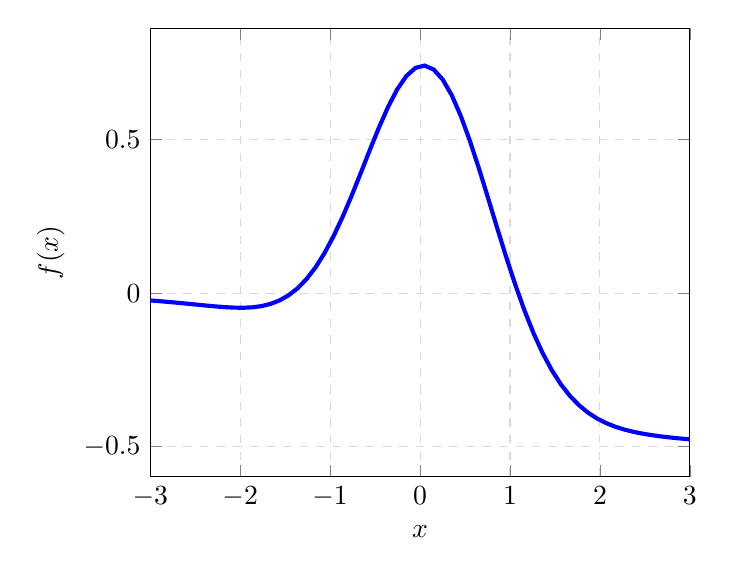
\begin{tikzpicture}
            \begin{axis}[
            grid=major, 
            grid style={dashed,gray!30},
            xlabel=$x$, % Set the labels
            ylabel=$f(x)$,
            xmin=-3,
            xmax=3]
            \addplot[mark=none,color=blue, line width=1.5pt, samples=100] {exp(-(x-0.1)^2)-0.5/(1+exp(-x))};%{exp(-x^2)-0.5*exp(-(x-2)^2)+1};
            \end{axis}
        \end{tikzpicture}
        \caption{Example of poor correspondence between local and global
        structure. If $x<0$ is initialized, gradient descent will lead us in
        negative direction of $x$. However, this leads away from the global optimum
        on the right.}
        \label{fig:Poor_correspondence}
    \end{center}
\end{figure}

Another issue may be that there even is no global minimum. This happens for
example with the usage of the softmax, where the weights are increased without
bound even when the accuracy is very good. This occurs because the actual labels
for the softmax can only approach 1 with larger values, but never actually reach
it.  On solution to the second phenomena would be label smoothing, where instead
of a hard 0-1 coding of the classification, each of the 0 are replaced by
$\frac{k}{\textrm{\# of output units }-1}$, and the label for the true
classification is replaced by $1-k$. The network is now able to
resemble the labels without extreme output values.


\subsubsection{Initialization strategies}\label{sub:Initialization_strategies}
In the last section, the poor correspondence between local and global structure
was shown. Initializations at the wrong place on the loss landscape lead to a
gradient descent in a direction away from the global optimum. But because we
don't know the shape of the loss landscape in advance, no initialization can
guarantee a good solution or even convergence at all. However, some strategies
seem to perform better than other and have become widely used.

The first and only known property of initialization is that is has to be
asymetric. This means that two units that share the same input must have
different weights attached to these inputs. If this is not the case, a
deterministic optimization algorithm will update both these parameters in the
same way. To break this symetry, the weights are initialized randomly. If a
gaussian or uniform distribution is used does not seem to matter.

However, the range of these functions is important. Wide distributions have a
stronger symetry breaking effect, but come with the risk of exploding gradients
as discussed in section \ref{sub:Vanishing_gradient}. The problem of vanishing
gradients arise if the distribution is too small. The statictical viewpoint
suggests a initialization to small weights nevertheless. Here, large weight
initialization is seen as a large gaussian prior on which and how the units
interact. As we have no reason to encourage one interaction over another, the
weights should be as small as possible. 

Some heuristics try to balance these different motivations. One of the most
famous one is the normalized initialization from Glorot
\cite{glorot2010understanding}. For a fully connected layer of $m$ inputs and
$n$ outputs, the weights should be initialized according to a uniform
distribution:

\begin{align}
    W \sim U(-\sqrt{\frac{6}{m+n}}, \sqrt{\frac{6}{m+n}})
\end{align}

The biases are normally initialized to a constant. A value of 0 seems to behave
well for most applications.




\subsubsection{Stopping criteria}\label{sub:Stopping_criteria}
In traditional optimization, simple heuristics are used to determine the point
of stopping, like a gradient of 0. However many local extrema exits on the loss
landscape of deep neural networks, making a stop at the first extremum
unattractable.

Therefore, other stopping criteria have been developed. What we normally see in
terms of performance is an initial decrease in training loss paired with an
increase in validation accuracy. But after some epochs, we enter the overfitting
region, where training loss keeps decreasing but validation accuracy also
decreases again. In early stopping, this is used the determine the stopping
point. After each epochs we store a copy of the parameter values. Then we train
the network for a fixed number of epochs. At the point when the validation error
starts to rise again, we can return to the parameter values from before. As no additional
computation time is required, this is a very efficient method from a
computational perspective, but may require some extra storage. This apporach is
very different to traditional optimization, as gradients may still be very large.



\subsection{Algorithms}
\subsubsection{Stochastic Gradient Descent}\label{SGD}
Stochastic Gradient Descent (SGD) is one of the most popular optimization
algorithm in deep learning. It is also one of the most basic ones, as it only
takes the gradient at the current position into account. In contrast to normal
gradient descent, SGD computes the gradient on minibatches, not on the whole
dataset. Nevertheless, as long as the training data is only used once, SGD gives
an unbiased estimate of the true gradient, see Section \ref{sub:Minibatch}. 

\begin{algorithm}
    \hypertarget{alg:SGD}{}
    \begin{algorithmic}[1]
        \caption{Stochastic gradient descent from \cite{Goodfellow-et-al-2016}}
        \REQUIRE learning rate $\lambda$
        \ENSURE a trained neural network
        \STATE initialize the network, dataset and training parameters
        \WHILE{stopping criteria is not met}
            \STATE sample minibatch of $m$ examples ${x^{(1)}, ... ,x^{(m)}}$
            \STATE compute gradient estimate $\hat{g}=\frac{1}{m} \nabla_\theta \sum_i L(f(x^{(i)};\theta),y^{(i)})$
            \STATE apply parameter update $\theta=\theta-\lambda\cdot\hat{g}$
        \ENDWHILE
        \STATE \textbf{return: the trained network}
    \end{algorithmic}
\end{algorithm}

First, the network is initialized. Then, the training loop repeats, until the
stopping criteria is met. At the beginning of each iteration, a minibatch is sampled. Then, the
gradients are calculated, multiplied by the learning rate $\lambda$ and finally
applied to update the parameter values.


\subsubsection{Learning rate decay}\label{sub:Learing_rate_decay}
One of the most important hyperparameters of SGD is the learning rate. While the
optimal learning rate differs for every problem, it is important to decay the
learning rate with the number of epochs. Initially, it is good to choose a large
learning rate. This leads to fast learning at the beginning, and avoids the
algorithm getting stuck in areas of high loss. As the number of epochs
increases, it is important to shrink the learning rate. Since SGD is a
stochastic algorithm, its gradient is inaccurate. Even when we find a local
minimum with a gradient of 0 on the minibatch, the true gradient will not be 0.
A small learning rate secures to get close to the minimum while not overshooting
it repeatedly.

How the learning rate is decayed varies from algorithm. A popular decay is
piecewise constant decay, where the learning rate is decayed by a constant
factor $\gamma$ after a fixed number of epochs.
\begin{align}
    lr = lr_0 \cdot \gamma^{\lfloor epoch/stepsize \rfloor}
\end{align}
Another popular algorithm is cosine decay, where the learning rate is decayed
continously.
\begin{align}\label{eq:cosine_decay}
    lr_t = lr_{min} + \frac{1}{2} (lr_{max} - lr_{min})(1+cos(\frac{T_{cur}}{T_0}\pi))
\end{align}
Here $lr_{min}$ and $lr_{max}$ define the range of the lr, $T_{cur}$
is the current and $T_0$ is the maximum number of epochs. The advantage of
cosine decay is that the learning rate is decayed down to 0 in the defined
interval, independent of the initial learning rate. In contrast, the smallest
learning rate of step decay is dependent of the initial one.

\subsubsection{SGD with Momentum}\label{sub:Momentum}
Momentum is a popular variation of SGD. It is used to speed up the training of
SGD. The term Momentum is used, as the underlying idea is the similar to the
physical context. Consider a frictionless ball rolling down a hill. The ball
builds up speed the further it rolls down by adding the acceleration of current
gradient to the velocity. The ball will speed up, until it faces an uphill,
where it will slow down again.

In context of deep learning, we use the velocity $v$ rather than only the
current gradient $g$ to update the parameters.

\begin{align}
    v_{t+1}=m \cdot v_t - \lambda g
\end{align}
Here, $m$ controls how strong the past gradient is taken into account, while
$\lambda$ denotes the current learning rate. For the ball to build up velocity,
it requires a constant downhill motion. The same is true for this case. The
gradient can only build up, if it points in the same direction for some
consecutive updates similar to the ball. Therefore, momentum speeds up the
gradients of parameters, whose gradient is constant in one direction over
multiple epochs. Parameters with alternating gradients for example will only
experience small updates, because the different orientations of their gradient
will level out. Formally, if parameter $p$ experiences the same gradient $g$
every time, it will reach a terminal velocity of
\begin{align}
    \frac{\lambda \lVert g \rVert}{1-m}
\end{align}
This also shows that $m$ can be used to control the speed up of the
training. If $\lambda$ is kept constant, the larger $m$, the faster
training will become, as long as the gradient is constant for multiple update
iterations. A value of $m=0.9$ for example would lead to a speed up factor of
$10$, while $m=0.8$ would lead to a speed up of $5$.

\begin{algorithm}
    \hypertarget{alg:SGD_Momentum}{}
    \begin{algorithmic}[1]
        \caption{Stochastic gradient descent with Momentum from \cite{qian1999momentum}}
        \REQUIRE learning rate $\lambda$
        \REQUIRE momentum parameter $m$
        \ENSURE a trained neural network
        \STATE initialize the network, dataset and training parameters
        \WHILE{stopping criteria is not met}
            \STATE sample minibatch of $m$ examples ${x^{(1)}, ... ,x^{(n)}}$
            \STATE compute gradient estimate $\hat{g}=\frac{1}{m} \nabla_\theta \sum_i L(f(x^{(i);\theta}),y^{(i)})$
            \STATE compute velocity update $v=m \cdot v - \lambda \hat{g}$
            \STATE apply parameter update $\theta=\theta-v$
        \ENDWHILE
        \STATE \textbf{return: the trained network}
    \end{algorithmic}
\end{algorithm}

In pseudo code, SGD with Momentum in ALgorithm \hyperlink{alg:SGD_Momentum}{2}
looks similar to normal SGD in ALgorithm \hyperlink{alg:SGD_Momentum}{1}. The
only difference is line 5 and 6, where the velocity is updated and then used to
update the parameters rather than the gradient itself.

\begin{comment}
Momentum also adds a regularization effect, because it is attracted to stable
or flat minima. If the minima is too small, it won't be able to stop the
momentum and therefore the SGD will move on. That's similar to a ball, which
won't stay in a small hole but keep on going, if it's speed is larger enough.
\end{comment}





\section{Related work}

The last sections focused on general challenges of neural network optimization
and how to overcome them. This section gets into more detail on some of these
and shows current techniques in neural network optimization, some of which are the basis
for the methods and results in the following chapters.




\subsection{Wide minima and Generalization}\label{sub:Generalization}
In section \ref{sub:1}, we saw how learning differs from normal optimization,
namely that we only have acces to the training set and thus have to optimize
indirectly. With an increasing number of training epochs, the network starts to
memorize the training data. Because the data distribution of the training data
is not identical to the distribution of test data, this usually leads to a
better performance of the network on the training set than on the test set. The
difference between those performances is known as Generalization Gap. 

Strategies that are developed to deal with this problem are subsumed under the
term \textbf{Regularization}. One common reguralizer is the $L_2$ Reguralizer.
Its goal is, to encourage the weights to stay small. Small weights have some
advantages for the generalization capabilities. First of all, small weights
remove the dependency of a unit to one of its inputs. Because the weights are
really small, a strong activation cannot be solely achieved by the presence of
one input, but rather has to rely on multiple units. Therefore small changes in
the input will only cause small changes in the output, instead of the absence of
one feature for example leading to a different output. This benefits the
generalization, as the distribution of training and test data is slightly
different. Formally this can be incorporated in the loss function by adding the
squared $L_2$ norm:
\begin{align}
    L= L(f(x;\theta), y)+l \cdot \lVert \theta \rVert_2^2
\end{align}
The paramter $l$ controls the strength of the $L_2$ and has to be adjusted individually
for each problem.

Other work has gone into understanding the connection to the loss surface.
Hochreiter \& Schmidhuber \cite{hochreiter1997flat} argued that flat minima
have better generalization capabilities. A flat minima is a region where the
loss stays constant in contrast to sharp one, where small steps can increase
the loss significantly. Therefore, flat minima will perform constantly even for
small changes in the input, whereas sharp minimas will lead to an increase in
generalization error. Support also comes from the minimum description length
theory, which states that fewer bits are needed to describe a flat minimum than
a sharp. Lower complexity leads to a better generalization error. The idea is,
that in the network we try to compress the data. The more we compress the data
while also beeing able to resemble it, the more of the structure of the data we
uncover. Therefore, a model with lower complexity can fit the underlying data
better and achieve a better generalization error. Keskar et al.
\cite{keskar2016large} draw the same conclusion. They also provide a solution
for finding flat minima in using small batch sizes, see chapter
\ref{sub:Minibatch}.

Work from Dinh et al. \cite{dinh2017sharp} however contradicts this view. They
argue that the notion of flat is problematic in the context of deep learning, as
the loss surface is very complex. Based on previous definitions from the
papers above, they construct parameter values which lie on a sharp point of the
surface, but are also able to generalize well. Therefore, at least some caution
is needed when arguing about flatness beeing a reason for generalization
capabilities.

\subsection{Loss landscape}\label{loss_landscape}
Section \ref{prob:5} showed that the poor correspondence between local
and global structure may propose a major issue for optimization. Bad
initializations may lead to path which moves away from the global otimum, often
without chance to recover. Initialization strategies try to adress this problem,
but cannot guarantee to solve it.

An open question is if this suboptimal structure is present in deep neural
networks. Fengxiang et al. \cite{he2020piecewise} showed that there exist
infinitly many local minima which are of higher cost than the global one.
Furthermore, these minima are arranged in enclosed areas, where each minima
within one area has the same loss as the others and is also connected to them by
paths of low loss. These areas are seperated from each other by
nondifferentiable boundaries. Unfortunally, it remains unclear if different areas 
are of different cost. If this is the case, this would propose a major problem.
When the training process gets into one of these areas, it is likely to get
stuck, probably in an area of suboptimal cost. A trivial way to recover is not
present at the moment.

Draxler et al. \cite{draxler2018essentially} get to a smiliar result, that local
minimas are connected by paths of low loss. On these paths, the training loss stays the
same to the one of the connected minima, while the test error rate slighly
increases.

Fort \& Jastrzebski \cite{fort2019large} put this in a more formal context. For
each tuple of dimensions, they construct disks to describe the hyperplanes
defined by them. They calls these hyperplanes wedges. One property is that the
paths of low loss described above lay on these wedges. Therefore the
connecting path for two points on different wedges has to pass through the
intersection of them, and their direct connection is an area of high loss.
When viewed from an cross-section, these paths from a tunnel. Some techniques
to improve optimization have similar effects on the size of these tunnels,
namely they widen them. This happens for example for higher $L_2$ regularization
\ref{sub:Generalization}, smaller batch sizes \ref{sub:Minibatch} or higher
learning rates.


\subsection{Cosine Decay with Warm Restart}\label{sub:cosine_decay}

In section \ref{SGD}, learning rate schedulers were introduced. The idea was to
have a high learning rate at the beginning for fast improvements, and then a
decrease to fine adjust the parameters. One scheduler was cosine decay, with the
formula \ref{eq:cosine_decay}. In the paper of Loshchilov \& Hutter
\cite{loshchilov2016sgdr}, they use this scheduler in combination with another
technique, called warm restart. In constrast to the naive approach, where the
learning rate is only decayed once, warm restart decayes until a fixed number of
epochs, and then set back up to the inital learning rate. This procedure can be
repeated for several times. The idea is, that a high learning rate leads to
exploration of the loss landscape, while a low learning rate leads to
exploitation.

In their results, at every restart, the performance becomes worse for some
epochs due to the high learning rate. But when the learning rate decays again, the
previous performance is reached and even topped. this leads to a new state of
the art result at 3.14\% test error for Wide-Residual-Net 28-20 on CIFAR-10.
Their method also perfoms better when compared to step decay. 


\subsection{Ensemble methods}\label{sub:Ensemble_Methods}
The general idea of ensemble methods is to combine the predictions of multiple
models to get a more accurate prediction. The fact that this leads to an
improvement can be seen in a simple regression problem. Suppose there exist $k$
models that make a prediction error of $e_i$ with mean 0, variance $E[e_i^2]=v$ and
covariances $E[e_i e_j]=c$ on every particular prediction. If these models are
combined, the variance reduces to 
\begin{align}
    E[(\frac{1}{k} \sum_i e_i)^2]=\frac{1}{k^2}E[\sum_i (e_i^2 + \sum_{j\neq i} e_i e_j)]=\frac{1}{k}v+\frac{k-1}{k}c
\end{align}
If all models make the same predictions, so $c=v$ for all combinations of
models, then the sum decomposes to $v$, so the prediction error is the same as
before. On the other hand, if $c=0$, the prediction error is reduced by a factor
of $\frac{1}{k}$. Therefore, for ensemble methods to be succesfull, every individual model
has to achieve a low prediction error, while the predictions of all models
should be as different as possible. While the low error is achieved in deep
learning by standard training of the models, there are several approaches to
ensure that the correlation between the models stays los.

The first idea would be to vary the training data for the model. One way this
can be realized is by k-fold cross-validation. Here, we split the training data
into $k$ different smaller datasets. Then we train $k$ independent networks on one
of these subsets. This however decreases the size of the training set for each
model drastically. Therefore another common approach is bagging
\cite{breiman1996bagging}, where we draw a subset from the training data, but
with replacement. Here, individual examples might occur in more than one
training set. Training on different datasets leads to lower correlation, which we
can use to our advantage as we have seen above. As the number of training
examples is limited however, we might not be able to sustain a sufficient low
error.

To use the whole training data while also creating different models, we can
alternatively alter the model itself. An naive approach would be to just use
different model architectures. If we want to use the same architecture for all
models, we can vary the parameter initilializations. This is often enough to
create models that have different predictions. However, for every initialization
a network has to be trained from beginning, which can become very costly. A
novel approach is to train one network, but to take snapshots of the network
parameters at different steps. This approach adds no additional cost, as we only
train one network. To ensure different networks, Huang et al.
\cite{huang2017snapshot} use the method of cosine decay with warm restarts
\cite{loshchilov2016sgdr}, as explained in section \ref{sub:cosine_decay}.
Recall that at each restart, the learning rate is set up to the initial learning
rate. This results in the optimizer taking larger update steps and consequently,
the network parameter values will distance from their current state. The
snapshots of the networks are taken before each restart, as the network
converges to area of low loss when the learning rate is low. With this method,
we are able to get models with low correlation, low error and no additional cost.

After we have ensured that the conditions for the models are met, we have to
think about how to combine threi predictions. For the case of classification
with the use of softmax layer, we can use a technique called model averaging.
Here, we sum the predictions of the individual models, and take the class with
the highest prediction, as in standard classification. Formally, if the
probability output of a model i for a given class c is $p_{c_i}$, then we sum
the probabilites of each individual model: $p_c = \sum_i p_{c_i}$. To predict
the class we take $argmax_c(p_c)$. If we have reasons to believe in a better
prediction of one model over another, we can add weights $w_i$ to the
probabilites of the individual models: $p_c = \sum_i w_i \cdot p_{c_i}$.


\begin{comment}
Further aspects that could be included:
- classififcation in general
- cross entropy loss and loss functions
- gradient descent
\end{comment}
\chapter{Methods}
\section{Distance Function}
\subsection{Motivation}
In chapter \ref{loss_landscape}, we got a brief overview over the loss landscape
of deep neural networks and the resulting challenges for optimization. Although
there exists a large number of local minima, most of them have low cost.
Furthermore, they are arranged in cells, where each minima has low cost and is
connected to the others via valleys of low loss.

These cells create a challenge for optimization. Suppose the learning gets into
the area of one of these cells. As mentioned in chapter \ref{loss_landscape} the
cells are surrounded by nondifferential boundaries and areas of higher loss.
[TODO: where is this stated?] This will likely cause the algorithm to get stuck
into this cells. As all of the minimas in this cell are of approximatly same
loss, there will be a boundary until the algorithm can improve, which may be
higher than the global optimum. This also poses the question, if continuing to
train is useful, as after one of the minima in the cell is found, the nearby
minima ic can reach will offer no significant improvement.

How to overcome this issue? One solution would be to escape these cells and move
to the next one, hopefully with lower cost. This can be achieved with the use of
warm restarts, as mentioned in chapter \ref{cosine_decay}. In phases of low
learning rate, the algorithm exploits the area of a cell. When the learning rate
is set back up to the inital learning rate, the update steps of the parameters
get much larger. If the update steps are large enough, this may lead to an
escape of the cell. However there is no guarantee, because this method relies on
the gradient beeing large enough.

From a naive point of view, it would be easiest to remember to place of the
cells, and just move away from it. In a simplified version, thats what our
algorithm does. It remembers the point which it wants to distance from, and then
rewards doing so. [describe better]
 
\begin{comment}
motivations:
- different values for ensemble method
- seen that cells exists, escape these cells
- explore instead of exploit

\end{comment}
\subsection{idea}
An easy approach to move away from an area would be to remember the point you
want to distance from, and then move in whatever direction increases this
distance. In a sense, this is what our algorithm does. It remembers the current
parameter values, and decreases the cost the further you are away from this
point. If one would only use this distance as a cost metric, it would be
successfull in distancing from the current checkpoint, but the learning would
stop. That's why we incooperate the distance term into the regular cost
function, to account for both the distance and the cost value.
\subsection{Mathematical apporach}
\subsubsection{Distance function}\label{distance_function}
As we want to measure the distance between two points, we need to define a
distance function. A common choice is the euclidean distance also know as $L_2$
norm, which is defined as: 
\begin{align}
    \rVert x \lVert_2 = \sqrt{\sum_i \lvert x_i \rvert^2}
\end{align}
This norm can also be squared to get rid of the root. Squaring does not change
the direction of the gradient, and is therefore possible. To measure the
distance between two parameter states $\theta_1$ and $\theta_2$ of the networks,
this results in:
\begin{align}\label{eq:distance}
    d(\theta_1, \theta_2)= \sum_i (\theta_{1_i}-\theta_{2_i})^2
\end{align}
The size and shape of the paramters $\theta$ is not important, as each paramter
is only compared to another state of itself, and is combined via a sum.

Another property is that the values the distance function can take is partly
dependend on size. Consider two networks $\theta_1$, $\theta_2$ with the same
classification task, but the size of $\theta_1$ is larger than $\theta_2$.[may
be confusing with before] If we assume all of the parameters are distributed the
same way, then $\theta_1$ would output a larger distance than $\theta_2$.
However it would be desirable for the functions to be in the same bound, as it
would make the transfer of hyperparameters for example possible. That's why we
use a function to control for the output to be in a certain bound.

If we take a look at support vector machines, they use kernels to compute the
similarity between two samples. One popular choice is the radial basis function
kernel, defined as:
\begin{align}
    k(\theta_1, \theta_2)=exp(-\frac{\rVert \theta_1 - \theta_2 \lVert^2}{2\sigma^2})
\end{align}
where $exp$ is the exponential function.
With the use of \ref{eq:distance}, we can convert this to:
\begin{align}
    k(\theta_1, \theta_2)=exp(-\frac{d(\theta_1, \theta_2)}{2\sigma^2})
\end{align}
This formulation has some nice properties. First of all, the values are now
bound between 0 an 1, regardless of the size f $\theta$. Second, we can see as
the values of the distance get larger, the function approaches 0 asymtotically.
This leads to a really small gradient for extreme distances. Consequently, the
Kernel will initially push the parameters away from the checkpoint, but when
this is achieved, will have little influence on the loss function. How far the
function encourages to distance from the checkpoint can be controlled by the
parameter $\sigma$, which defines the width of the function and can be tuned as
a hyperparamter.


\subsubsection{Loss function}
This section will show how the distance function from \ref{distance_function} is
combined with the normal loss function. The state of the art loss function for
image classification, which will be used for testing is the cross-entropy-loss
defined as:
\begin{align}
    -\sum_{c} \delta_{yc} log(f(x)_c)
\end{align}
Where $\delta$ is the Kronecker-Delta function defined as:
\begin{align}
    \delta_{xy} =
    \begin{cases}
        1 \textrm{, if } x=y \\
        0 \textrm{ otherwise}
    \end{cases}
\end{align}

To account for the distance term, we just sum it with the cross-entropy-loss:
\begin{align}
    L=\sum_{c} \delta_{yc} log(f(x)_c) + distance(\theta, \theta_c)
\end{align}
When computing the derivative for the backpropagation, the sum decomposes into
two terms, so the cross-entropy-loss will be computed the same as before.
Another property we want to control for is the influence of the distance versus
the cross-entropy-loss. When training is in later stages, the cross-entropy-loss
may be very small. If the values of the distance function a too large in
comparison, this would cause the parameters to be updated only based on the
distance, which is undesirable as the performance wouldn't be taken into account
anymore. The same is also true the other way around, if the distance function is
too small, it wouldn't affect training at all. That's why we introduce a
hyperparameters $w$ called weight to control this:
\begin{align}
    L=\sum_{c} \delta_{yc} log(f(x)_c) + w \cdot distance(\theta, \theta_c)
\end{align}

\subsection{Pytorch implementation}

\subsubsection{Checkpoint creation}
To measure the distance, we have to create the checkpoint. The model parameters
in pytorch are stored as matrices for each layer and can be accesed via
$model.parameters()$, which outputs an iterable. We therefore opt to keep this
structure and safe the parameters in a list.
\begin{algorithm}[htbp]
    \caption{Checkpoint}\label{alg:Checkpoint}
    \lstset{language=Python}
    \lstinputlisting{src/createCheckpoint.py}
\end{algorithm}
\newline
First, the checkpoint list is initialized. Then we iterate over the model
parameters. For each layer, we have to clone the parameters in order to create
new variables, and not just pointers to the existing ones. In addition they have
to be detached, to remove connection of the gradient to the model parameters.

\subsubsection{Distance function}
The L2 norm is implemented the follwing way: We iterate over the checkpoint and
the current parameter values. For each layer, we compute the difference, and
then square and add the values to our distance.
\begin{algorithm}[htbp]
    \caption{L2 norm}\label{alg:L2Norm}
    \lstset{language=Python}
    \lstinputlisting{src/L2.py}
\end{algorithm}



\section{Configuration}

\subsection{Library and Training}
describe pytorch and the training loop

\subsection{datasets}
describe the used datasets
\subsection{Networks}
Describe the networks that are used,
mention pramaters that are fixed (like SGD) here and variables in the results part??
\subsection{hardware}
describe hardware used, cluster etc??

\chapter{Results}
After the theoretical introduction in chapter \ref{cha:Methods}, this chapter
provides some empirical results. In section \ref{res:baseline}, a baseline for
further comparisons will be created. Section \ref{res:Hyperparameters} will
focus on the effects of the hyperparameters of the distance function. How
multiple checkpoints can be used will section \ref{res:Multiple}show, followed
by the combination with learning rate schedulers \ref{res:Learning_rate}. We
will investigate the effects on ensemble methods in section \ref{res:Ensemble}
and finally study the computational cost in \ref{Res:Computational_cost}.



\section{Baseline}\label{res:Baseline} For the baseline, we use the
hyperparameters as defined in section \ref{sub:Hyperparameters}. First we train
both networks without distance function. After 100 epochs, we add a checkpoint
in the case of the network with distance function.

For the validation accuray, we can see no impact of the distance function.Both
networks show a standard learning curve, with a initial strong increase in
validation accuracy until coming into convergence in later epochs. This results
in a validation accuracy of arounf 90\% for MobileNetV2 and 89\% for ResNet32
after 600 epochs.



If we plot the distance the network gets to the checkpoint however, we can see
that the network trained with distance function clearly increases its distance
more than the one trained without. Furthermore, the red plot follows the shape
we would expect from the distance function. At the beginning, the distance
increases relatively fast, as can be expected from the high gradient of the RBF
Kernel. But as the distance increases, its gradient becomes smaller, similar to
the gradient of the Kernel. The blue plot in contrast follows an almost linear
curve, whith a much smaller gradient. Therefore, the additional term succeeds in
the initial goal, which was to distance from the checkpoint. Note that despite
the validation accuracy beeing in an area of convergence, SGD even without
distance function keeps on walking and never truly stops at a point.

\begin{figure}[h]\label{fig:Results_baseline}
    \begin{center}
        \begin{tikzpicture}
            \begin{groupplot}[
                group style={
                group size=2 by 2,
                horizontal sep=10pt,
                vertical sep=10pt,
                group name=G},
                width=8cm,
            ]

            \nextgroupplot[
            grid=major, 
            grid style={dashed,gray!30},
            % xlabel=Epoch,
            ylabel=Validation Accuracy,
            xticklabels={,,},
            ymin=0.8,
            xmin=-10]
            \addplot[mark=None, color=red] 
                table[x=Step, y=Value, col sep=comma]{images/network_csv/baseline/MobileNetV2/MobileNetV2_baseline_validation_acuracy.csv};
            \addplot[mark=None, color=blue] 
                table[x=Step, y=Value, col sep=comma]{images/network_csv/baseline/MobileNetV2/MobileNetV2_baseline_distance_validation_acuracy.csv};
            
            \nextgroupplot[
                grid=major, 
                grid style={dashed,gray!30},
                % xlabel=Epoch,
                ylabel=Distance,
                yticklabel pos=right,
                xticklabels={,,},
                ylabel near ticks]
                \addplot[mark=None, color=red] 
                    table[x=Step, y=Value, col sep=comma]{images/network_csv/baseline/MobileNetV2/MobileNetV2_baseline_distance0.csv};
                \addplot[mark=None, color=blue] 
                    table[x=Step, y=Value, col sep=comma]{images/network_csv/baseline/MobileNetV2/MobileNetV2_baseline_distance_distance0.csv};
    

            \nextgroupplot[
            grid=major, 
            grid style={dashed,gray!30},
            xlabel=Epoch, % Set the labels
            ylabel=Validation Accuracy,
            ymin=0.8,
            xmin=-10]
            \addplot[mark=None, color=red] 
                table[x=Step, y=Value, col sep=comma]{images/network_csv/baseline/ResNet32/ResNet32_baseline_validation_acuracy.csv};
            \addplot[mark=None, color=blue] 
                table[x=Step, y=Value, col sep=comma]{images/network_csv/baseline/ResNet32/ResNet32_baseline_distance_validation_acuracy.csv};
            
            \nextgroupplot[
                grid=major, 
                grid style={dashed,gray!30},
                xlabel=Epoch, % Set the labels
                ylabel=Distance,
                yticklabel pos=right,
                ylabel near ticks]
                \addplot[mark=None, color=red] 
                    table[x=Step, y=Value, col sep=comma]{images/network_csv/baseline/ResNet32/ResNet32_baseline_distance0.csv};
                \addplot[mark=None, color=blue] 
                    table[x=Step, y=Value, col sep=comma]{images/network_csv/baseline/ResNet32/ResNet32_baseline_distance_distance0.csv};

            \end{groupplot}
        \end{tikzpicture}
        \caption{Validation accuray and distance to the checkpoint for MobileNetV2 (upper) and ResNet32 (lower) trained without distance function (red) and with distance function (blue).}
    \end{center}
\end{figure}


[TODO: add gradient size to show that circular path]




\section{Distance function Hyperparameters}\label{res:Hyperparameters}
\subsection{strength}
Recall section \ref{eq:Loss_strength}, where we added strength as a
hyperparameter, controlling the influence of the distance function. As the RBF
Kernel is bound between 0 and 1, the strength hyperparameter will increase that
bound between 0 and the strength value.

For higher strength values, the validation accuracy receives an initial drop
after a checkpiont is added, which is larger the higher the strength parameter
value, see figure \ref{fig:Results_strength}. This may be due to the increased
influence of the strength function. Each distance between the parameters and the
checkpoint starts at 0, therefore the values of the exponential function starts
at $strength \cdot 1$. A higher strength value will lead to a higher influence
on the loss function, and consequently on the gradient. The gradient of the
cross-entropy loss will become insignificant, and the optimizer will update the
weights without regards to the validation accuracy, hence the drop at the
beginning. 

The distance plot reflects this behaviour, as we can see an larger increase in
distance for larger strength values. After the initial step however, the
distance quickly converges. This is due to the fact that after the initial
strong decrease, the value of the distance function quickly comes close to 0.
Therefore, the distance Kernel becomes insignificant again, and the
Cross-Entropy loss is followed. The validation accuracy reflects this behaviour,
as after the initial drop the accuracy recovers to the level of before. This
provides additional insight in the loss landscape. As the network distances from
it`s current position on the loss landscpae, but is still able to reach high
accuracy, there have to be areas of high accuracy everywhere on the landscape.
This is in consonance to other research in this field, as discussed in section
\ref{loss_landscape}.

As a result, the value of the strength doesn't matter in long term at least. It
merely increases the distance to the checkpoint by defining how long the
distance term is important to the loss function. But after that, the normal loss
is followed again. As the last section and literature suggests, area of low loss
and high accuray can be found everywhere. Therefore, the same accuracy as before
can be reached, no matter the value of the strength. On the other hand, it is
also unlikely that it will outperform the last best value, as new areas are not
generally better than other. That's why the effect of the distance doesn't
transfer to the validation accuracy.



\begin{figure}[h]\label{fig:Results_strength}
    \begin{center}
        \begin{tikzpicture}
            \begin{groupplot}[
                group style={
                group size=2 by 2,
                horizontal sep=10pt,
                vertical sep=10pt,
                group name=G},
                width=8cm,
                restrict x to domain=0:200
            ]

            \nextgroupplot[
            grid=major, 
            grid style={dashed,gray!30},
            % xlabel=Epoch,
            y label style={at={(axis description cs:0.1,0)},anchor=south},
            ylabel=Validation Accuracy,
            xticklabels={,,},
            ymin=0.6,
            legend pos= south east,
            xmin=-10]
            \addplot[mark=None, color=red] 
                table[x=Step, y=Value, col sep=comma]{images/network_csv/strength/MobileNetV2/MobileNetV2_strength_e1_validation_acuracy.csv};
            \addlegendentry{$s=0.1$}
            \addplot[mark=None, color=blue] 
                table[x=Step, y=Value, col sep=comma]{images/network_csv/baseline/MobileNetV2/MobileNetV2_baseline_distance_validation_acuracy.csv};
            \addlegendentry{$s=1$}
            \addplot[mark=None, color=orange] 
                table[x=Step, y=Value, col sep=comma]{images/network_csv/strength/MobileNetV2/MobileNetV2_strength_e2_validation_acuracy.csv};
            \addlegendentry{$s=10$}
            \addplot[mark=None, color=green] 
                table[x=Step, y=Value, col sep=comma]{images/network_csv/strength/MobileNetV2/MobileNetV2_strength_e3_validation_acuracy.csv};
            \addlegendentry{$s=100$}

            \nextgroupplot[
                grid=major, 
                grid style={dashed,gray!30},
                % xlabel=Epoch,
                y label style={at={(-0.1,0.5)},anchor=south},
                ylabel=Distance,
                yticklabel pos=right,
%                y label style={at={(axis description cs:0,0)},anchor=south},
                xticklabels={,,},
                ylabel near ticks]
            \addplot[mark=None, color=red] 
                table[x=Step, y=Value, col sep=comma]{images/network_csv/strength/MobileNetV2/MobileNetV2_strength_e1_distance0.csv};
            \addplot[mark=None, color=blue] 
                table[x=Step, y=Value, col sep=comma]{images/network_csv/baseline/MobileNetV2/MobileNetV2_baseline_distance_distance0.csv};
            \addplot[mark=None, color=orange] 
                table[x=Step, y=Value, col sep=comma]{images/network_csv/strength/MobileNetV2/MobileNetV2_strength_e2_distance0.csv};
            \addplot[mark=None, color=green] 
                table[x=Step, y=Value, col sep=comma]{images/network_csv/strength/MobileNetV2/MobileNetV2_strength_e3_distance0.csv};
    

            \nextgroupplot[
            grid=major, 
            grid style={dashed,gray!30},
            % x label style={at={(axis description cs:1.5,0)},anchor=west},
            xlabel=Epoch, % Set the labels
            % ylabel=Validation Accuracy,
            ymin=0.6,
            xmin=-10]
            \addplot[mark=None, color=red] 
                table[x=Step, y=Value, col sep=comma]{images/network_csv/strength/ResNet32/ResNet32_strength_e1_validation_acuracy.csv};
            \addplot[mark=None, color=blue] 
                table[x=Step, y=Value, col sep=comma]{images/network_csv/baseline/ResNet32/ResNet32_baseline_distance_validation_acuracy.csv};
            \addplot[mark=None, color=orange] 
                table[x=Step, y=Value, col sep=comma]{images/network_csv/strength/ResNet32/ResNet32_strength_e2_validation_acuracy.csv};
            \addplot[mark=None, color=green] 
                table[x=Step, y=Value, col sep=comma]{images/network_csv/strength/ResNet32/ResNet32_strength_e3_validation_acuracy.csv};
            
            \nextgroupplot[
                grid=major, 
                grid style={dashed,gray!30},
                %xlabel=Epoch, % Set the labels
                %ylabel=Distance,
                yticklabel pos=right,
                ylabel near ticks]
            \addplot[mark=None, color=red] 
                table[x=Step, y=Value, col sep=comma]{images/network_csv/strength/ResNet32/ResNet32_strength_e1_distance0.csv};
            \addplot[mark=None, color=blue] 
                table[x=Step, y=Value, col sep=comma]{images/network_csv/baseline/ResNet32/ResNet32_baseline_distance_distance0.csv};
            \addplot[mark=None, color=orange] 
                table[x=Step, y=Value, col sep=comma]{images/network_csv/strength/ResNet32/ResNet32_strength_e2_distance0.csv};
            \addplot[mark=None, color=green] 
                table[x=Step, y=Value, col sep=comma]{images/network_csv/strength/ResNet32/ResNet32_strength_e3_distance0.csv};

            \end{groupplot}
        \end{tikzpicture}
        \caption{Validation accuracy and Distance for MobileNetV2 (upper) and ResNet32 (lower) trained without distance function and different strength values.}
    \end{center}
\end{figure}

\subsection{width}
We have seen in chapter \ref{distance_function}, how the width $\sigma$
influences the distance function: The larger $\sigma$ gets, the wider it
becomes. Therefore, a larger $\sigma$ should result in the network distancing
further from it's checkpoint than for smaller values. That's exactly what can be
seen in figure \ref{fig:Results_width}: For an $\sigma^2$ of 0.1, the distance
follows the one of network trained without distance function, due to the
distance function quickly becoming 0 and therefore having no influence. The
larger the width, the slower the values of the distance function decrease for further
distance. Therefore, the gradient of the distance function will stay quite
large, pushing the network further away. This can be seen for higher $\sigma$
values, where the distance increases further.


Initially however, the distance plot doesn't reflect this behaviour. The curve
for $\sigma = 0.01$ has a higher distance value than for $\sigma = 0.001$.
That's because the gradient of the distance function is higher for small distances, the
smaller $\sigma$. But for larger distances, this effect flips with the gradient
of the larger width staying higher for more epochs. Therefore, the curves
intersect after additional epochs. The smaller width converges, while the larger
stays constant until eventually reaching it`s area of convergence. The
intersection happens later the larger the width, for $\sigma = 0.0001$, only
after 207 epochs.

This behaviour however has no influence on the validation accuracy, which stays
the same for every width, in contrast to the strength. This may be due to the
fact, that a larger width does in fact decreases the size of the gradient. A
smaller gradient over more epochs will be added to the gradient of the
Cross-Entropy Loss. The optimizer therefore nearly keeps on following the normal
gradient and descending the valley of low loss, with a small but steady push to
increase the distance to the checkpoint. Therefore, even if the network is
allowed to move quite freely on the loss surface, it finds areas of low loss and
high accuracy in distant areas of the checkpiont, meaning there has to be good
local minima everywhere on the landscape.

In particular, $\sigma^2 = 100$ seems to increase the distance far enough in a
small number of epochs. That's why this configuration is used as standard in the
following work.

\begin{figure}[h]\label{fig:Results_width}
    \begin{center}
        \begin{tikzpicture}
            \begin{groupplot}[
                group style={
                group size=2 by 2,
                horizontal sep=10pt,
                vertical sep=10pt,
                group name=G},
                width=8cm,
                restrict x to domain=0:400
            ]

            \nextgroupplot[
            grid=major, 
            grid style={dashed,gray!30},
            % xlabel=Epoch,
            ylabel=Validation Accuracy,
            xticklabels={,,},
            ymin=0.7,
            legend pos = south east,
            xmin=-10]
            \addplot[mark=None, color=red] 
                table[x=Step, y=Value, col sep=comma]{images/network_csv/width/MobileNetV2/MobileNetV2_width_e1_validation_acuracy.csv};
            \addlegendentry{$\sigma^2=1$}
            \addplot[mark=None, color=orange] 
                table[x=Step, y=Value, col sep=comma]{images/network_csv/width/MobileNetV2/MobileNetV2_width_e2_validation_acuracy.csv};
            \addlegendentry{$\sigma^2=10$}
            \addplot[mark=None, color=blue]
                table[x=Step, y=Value, col sep=comma]{images/network_csv/baseline/MobileNetV2/MobileNetV2_baseline_distance_validation_acuracy.csv};
            \addlegendentry{$\sigma^2=100$}
            \addplot[mark=None, color=green] 
                table[x=Step, y=Value, col sep=comma]{images/network_csv/width/MobileNetV2/MobileNetV2_width_e4_validation_acuracy.csv};
            \addlegendentry{$\sigma^2=1000$}

            \nextgroupplot[
                grid=major, 
                grid style={dashed,gray!30},
                % xlabel=Epoch,
                ylabel=Distance,
                yticklabel pos=right,
                xticklabels={,,},
                ylabel near ticks]
            \addplot[mark=None, color=red] 
                table[x=Step, y=Value, col sep=comma]{images/network_csv/width/MobileNetV2/MobileNetV2_width_e1_distance0.csv};
            \addplot[mark=None, color=orange] 
                table[x=Step, y=Value, col sep=comma]{images/network_csv/width/MobileNetV2/MobileNetV2_width_e2_distance0.csv};
            \addplot[mark=None, color=blue] 
                table[x=Step, y=Value, col sep=comma]{images/network_csv/baseline/MobileNetV2/MobileNetV2_baseline_distance_distance0.csv};
            \addplot[mark=None, color=green] 
                table[x=Step, y=Value, col sep=comma]{images/network_csv/width/MobileNetV2/MobileNetV2_width_e4_distance0.csv};
    

            \nextgroupplot[
            grid=major, 
            grid style={dashed,gray!30},
            xlabel=Epoch, % Set the labels
            ylabel=Validation Accuracy,
            ymin=0.7,
            xmin=-10]
            \addplot[mark=None, color=red] 
                table[x=Step, y=Value, col sep=comma]{images/network_csv/width/ResNet32/ResNet32_width_e1_validation_acuracy.csv};
            \addplot[mark=None, color=orange] 
                table[x=Step, y=Value, col sep=comma]{images/network_csv/width/ResNet32/ResNet32_width_e2_validation_acuracy.csv};
            \addplot[mark=None, color=blue] 
                table[x=Step, y=Value, col sep=comma]{images/network_csv/baseline/ResNet32/ResNet32_baseline_distance_validation_acuracy.csv};
            \addplot[mark=None, color=green] 
                table[x=Step, y=Value, col sep=comma]{images/network_csv/width/ResNet32/ResNet32_width_e4_validation_acuracy.csv};

            
            \nextgroupplot[
                grid=major, 
                grid style={dashed,gray!30},
                xlabel=Epoch, % Set the labels
                ylabel=Distance,
                yticklabel pos=right,
                ylabel near ticks]
            \addplot[mark=None, color=red] 
                table[x=Step, y=Value, col sep=comma]{images/network_csv/width/ResNet32/ResNet32_width_e1_distance0.csv};
            \addplot[mark=None, color=orange] 
                table[x=Step, y=Value, col sep=comma]{images/network_csv/width/ResNet32/ResNet32_width_e2_distance0.csv};
            \addplot[mark=None, color=blue] 
                table[x=Step, y=Value, col sep=comma]{images/network_csv/baseline/ResNet32/ResNet32_baseline_distance_distance0.csv};
            \addplot[mark=None, color=green] 
                table[x=Step, y=Value, col sep=comma]{images/network_csv/width/ResNet32/ResNet32_width_e4_distance0.csv};

            \end{groupplot}
        \end{tikzpicture}
        \caption{Validation accuray and Distance for MobileNetV2 (upper) and ResNet32 (lower) trained with different widths of the distance function.}
    \end{center}
\end{figure}



\section{Multiple Checkpoint}\label{res:Multiple} In chapter \ref{cha:Methods},
we have seen that we can not only incorporate one but also multiple checkpoints
in the loss function, on which this section will focus. We also try to not only
add these checkpoints as seperate terms, but rather incorporate them in one
larger checkpoint. 

\subsection{multiple}
We add a checkpoint after every 150 epochs that are performed, resulting in a
total of 3 checkpoints after 600 epochs.

For the validation accuracy, we can see the same pattern as in section
\ref{res:Hyperparameters}. For low strength, we experience no effect at all. If
we increase the strength there is an initial drop in the accuracy. For
MobileNetV2, the accuracy recovers and even tops the baseline, with a small but
increasing margin for every new checkpoints that is added, coming to an
improvement of 0.8\% over the baseline after 600 epochs. In contrast, ResNet32
doesn't seem to benefit from multiple checkpoints, the accuracy even decreases
for larger strength values.

The pattern of MobileNetV2 is quite similar to warm restarts, where for every
restart the reached accuracy increases. For a in depth comparison, see section
\ref{res:Learning rate}.

\begin{figure}[h]\label{fig:Results_multiple}
    \begin{center}
        \begin{tikzpicture}
            \begin{groupplot}[
                group style={
                group size=2 by 1,
                horizontal sep=10pt,
                vertical sep=10pt,
                group name=G},
                width=8cm
            ]

            \nextgroupplot[
            grid=major, 
            grid style={dashed,gray!30},
            xlabel=Epoch,
            ylabel=Validation Accuracy,
            ymin=0.6,
            ymax=1,
            legend pos = south east,
            xmin=-10]
            \addplot[mark=None, color=red] 
                table[x=Step, y=Value, col sep=comma]{images/network_csv/multiple/MobileNetV2/MobileNetV2_multiple_validation_acuracy.csv};
                \addlegendentry{$s=1$}
            \addplot[mark=None, color=green] 
                table[x=Step, y=Value, col sep=comma]{images/network_csv/multiple/MobileNetV2/MobileNetV2_multiple_f10_validation_acuracy.csv};
                \addlegendentry{$s=10$}
            \addplot[mark=None, color=blue] 
                table[x=Step, y=Value, col sep=comma]{images/network_csv/multiple/MobileNetV2/MobileNetV2_multiple_f100_validation_acuracy.csv};
                \addlegendentry{$s=100$}
            
    

            \nextgroupplot[
            grid=major, 
            grid style={dashed,gray!30},
            xlabel=Epoch, % Set the labels
            ytick pos=right,
            ymin=0.6,
            ymax=1,
            xmin=-10]
            \addplot[mark=None, color=red] 
                table[x=Step, y=Value, col sep=comma]{images/network_csv/multiple/ResNet32/ResNet32_multiple_validation_acuracy.csv};
            \addplot[mark=None, color=green] 
                table[x=Step, y=Value, col sep=comma]{images/network_csv/multiple/ResNet32/ResNet32_multiple_f10_validation_acuracy.csv};
            \addplot[mark=None, color=blue] 
                table[x=Step, y=Value, col sep=comma]{images/network_csv/multiple/ResNet32/ResNet32_multiple_f100_validation_acuracy.csv};
            % [TODO: add ResNet Multiple]

            \end{groupplot}
        \end{tikzpicture}
        \caption{Validation accuray and Distance for MobileNetV2 (upper) and ResNet32 (lower) trained with multiple checkpoints. [TODO: add for ResNet]}
    \end{center}
\end{figure}

The influence on the distance to the checkpoints is more interesting however. In
general, an additional checkpoint seems to decrease the distance to the others.
This is quite counterintuitive at first glance. Suppose for one parameter, we
have checkpoint value $a$ and create a new one at our current value $b<a$. To
increase the distance to both, we would just have to walk in direction $c<b$. As
we have seen in previous section, this would be sufficient as areas of low error
exist everywhere. But why is the distance then decreased for our first
checkpoint? The reason might be the $L_2$ regularization, as it restricts the
weights to small sizes. At some point, it might be less costly to decrease the
weights again for a smaller $L_2$, traded off against a bit smaller distance to
other checkpoints. This restriction in weight space is probably why new terms
lead to a decrease of the distance to existing checkpoints. A network trained
without $L_2$ regularization futher supports this explanation. Here, the
distance increases further for each new checkpoint that is added. [add figure??]

\begin{figure}[h]\label{fig:Results_multiple_distance}
    \begin{center}
        \begin{tikzpicture}
            \begin{groupplot}[
                group style={
                group size=3 by 2,
                horizontal sep=10pt,
                vertical sep=10pt,
                group name=G},
                width=5cm
            ]

            \nextgroupplot[
            title=checkpoint 1,
            grid=major, 
            grid style={dashed,gray!30},
            %x label style={at={(axis description cs:1.5,0)},anchor=north},
            % y label style={at={(axis description cs:-0.1,.5)},rotate=90,anchor=south},
            %xlabel=Epoch,
            ylabel=distance,
            ylabel near ticks,
            ymax=8000,
            xmin=140,
            xticklabels={,,}]
            \addplot[mark=None, color=red] 
                table[x=Step, y=Value, col sep=comma]{images/network_csv/multiple/MobileNetV2/MobileNetV2_multiple_distance0.csv};
            \addplot[mark=None, color=green] 
                table[x=Step, y=Value, col sep=comma]{images/network_csv/multiple/MobileNetV2/MobileNetV2_multiple_f10_distance0.csv};
            \addplot[mark=None, color=blue] 
                table[x=Step, y=Value, col sep=comma]{images/network_csv/multiple/MobileNetV2/MobileNetV2_multiple_f100_distance0.csv};

            \nextgroupplot[
            title=checkpoint 2,
            grid=major, 
            grid style={dashed,gray!30},
            yticklabels={,,}
            ymax=8000,
            xmin=290,
            xticklabels={,,}]
            \addplot[mark=None, color=red] 
                table[x=Step, y=Value, col sep=comma]{images/network_csv/multiple/MobileNetV2/MobileNetV2_multiple_distance1.csv};
            \addplot[mark=None, color=green] 
                table[x=Step, y=Value, col sep=comma]{images/network_csv/multiple/MobileNetV2/MobileNetV2_multiple_f10_distance1.csv};
            \addplot[mark=None, color=blue] 
                table[x=Step, y=Value, col sep=comma]{images/network_csv/multiple/MobileNetV2/MobileNetV2_multiple_f100_distance1.csv};

            \nextgroupplot[
            title=checkpoint 3,
            grid=major, 
            grid style={dashed,gray!30},
            yticklabels={,,},
            ymax=8000,
            legend pos = outer north east,
            xmin=440,
            xticklabels={,,}]
            \addplot[mark=None, color=red] 
                table[x=Step, y=Value, col sep=comma]{images/network_csv/multiple/MobileNetV2/MobileNetV2_multiple_distance2.csv};
                \addlegendentry{$s=1$}
            \addplot[mark=None, color=green] 
                table[x=Step, y=Value, col sep=comma]{images/network_csv/multiple/MobileNetV2/MobileNetV2_multiple_f10_distance2.csv};
                \addlegendentry{$s=10$}
            \addplot[mark=None, color=blue] 
                table[x=Step, y=Value, col sep=comma]{images/network_csv/multiple/MobileNetV2/MobileNetV2_multiple_f100_distance2.csv};
                \addlegendentry{$s=100$}

%--------------------ResNet----------------------------------------------------

            \nextgroupplot[
            grid=major, 
            grid style={dashed,gray!30},
            ylabel=distance,
            ylabel near ticks,
            ymax=8000,
            xmin=140]
            \addplot[mark=None, color=red] 
                table[x=Step, y=Value, col sep=comma]{images/network_csv/multiple/ResNet32/ResNet32_multiple_distance0.csv};
            \addplot[mark=None, color=green] 
                table[x=Step, y=Value, col sep=comma]{images/network_csv/multiple/ResNet32/ResNet32_multiple_f10_distance0.csv};
            \addplot[mark=None, color=blue] 
                table[x=Step, y=Value, col sep=comma]{images/network_csv/multiple/ResNet32/ResNet32_multiple_f100_distance0.csv};

            \nextgroupplot[
            grid=major, 
            grid style={dashed,gray!30},
            xlabel=Epoch,
            yticklabels={,,}
            ymax=8000,
            xmin=290]
            \addplot[mark=None, color=red] 
                table[x=Step, y=Value, col sep=comma]{images/network_csv/multiple/ResNet32/ResNet32_multiple_distance1.csv};
            \addplot[mark=None, color=green] 
                table[x=Step, y=Value, col sep=comma]{images/network_csv/multiple/ResNet32/ResNet32_multiple_f10_distance1.csv};
            \addplot[mark=None, color=blue] 
                table[x=Step, y=Value, col sep=comma]{images/network_csv/multiple/ResNet32/ResNet32_multiple_f100_distance1.csv};

            \nextgroupplot[
            grid=major, 
            grid style={dashed,gray!30},
            yticklabels={,,},
            ymax=8000,
            xmin=440]
            \addplot[mark=None, color=red] 
                table[x=Step, y=Value, col sep=comma]{images/network_csv/multiple/ResNet32/ResNet32_multiple_distance2.csv};
            \addplot[mark=None, color=green] 
                table[x=Step, y=Value, col sep=comma]{images/network_csv/multiple/ResNet32/ResNet32_multiple_f10_distance2.csv};
            \addplot[mark=None, color=blue] 
                table[x=Step, y=Value, col sep=comma]{images/network_csv/multiple/ResNet32/ResNet32_multiple_f100_distance2.csv};

            \end{groupplot}
        \end{tikzpicture}
        \caption{Distance plots for MobileNetV2 (upper) and ResNet32 (lower) trained with multiple checkpoints and different strength values. [TODO: add for ResNet]}
    \end{center}
\end{figure}

In short term however, new checkpoint produce quite different influence on the
distance to existing ones. For a strength of $s=1$ we can see a slight decrease
which turns into a longer increase until the next checkpoint. For $s=10$, we see
an aprupt decrease with an small peak after. For $s=100$, there only is a peak
at the beginning which quickly diminishes. Noticeable, this pattern repeats for
the other checkpoints and therefore seems unlikely to be a coincidence. The size
of these hills can be tracked to the size of the strength. Larger strength
introduces a larger gradient and therefore step size at the beginning, making
the hills larger. This doesn't explain the different orientation of these hills.
For the case of $s=100$, the initial increase of distance seems reasonable. As
the value of the old distance function is not 0 when a new checkpoints is
created, the current gradient should face in direction away from the last
checkpoint. A new checkpoint term in the loss function introduces a gradient
boost, as section \ref{sub:Effect_on_Gradient} discussed. Because momentum
preserves the old gradient, it will acclerate in direction away from the first
and the second checkpoint, therefore leading to a hill. However by this
explanation, the pattern should repeat for the other strength values, which is
not the case. Therefore, the true cause of the short term effects remains
unclear.


- gradient size becomes smaller for distance term -> maybe hint that SGD wants
to stay in that area and distance term tries to push out -> gradient direction
would be interesting (but too far for this work)

\subsection{merge}
A slightly different approach is to merge the checkpoints, described in section
\ref{sub:Multiple_checkpoints}.
[TODO: add more networks for merge]










\section{lr}\label{res:Learning_rate}
\subsection{Scheduler}
Learning rate Scheduler were introduced in section \ref{sub:Learing_rate_decay},
where the learning rate was not held constant, but decayed over time. One
further addition were warm restarts, where after the decay we set the learning
rate back up to the inital and repeat this cycle several times. We use a step
decay scheduler with $\gamma = 0.1$ for every 50 epochs, and a warm restart
after 150 epochs. For cosine decay with warm restart, we set $\epsilon_{min}=0$,
$\epsilon_{max}=0.001$ and $T_0=150$.


For the validation accuracy, we can see that schedulers outperform a fixed
learning rate. At the beginning of every cycle, the performance drops due to
high learning rate. But when the learning rate decays again, the accuracy
recovers. Furthermore, the maximum accuracy of every cycle slightly increases,
until eventually coming to convergence. This leads to a maximum accuracy of
around 95\% for both ResNet32 and MobileNetV2.


\begin{figure}[h]\label{fig:Results_scheduler}
    \begin{center}
        \begin{tikzpicture}
            \begin{groupplot}[
                group style={
                group size=2 by 2,
                horizontal sep=10pt,
                vertical sep=10pt,
                group name=G},
                width=8cm
            ]

            \nextgroupplot[
            grid=major, 
            grid style={dashed,gray!30},
            % xlabel=Epoch,
            ylabel=Validation Accuracy,
            xticklabels={,,},
            ymin=0.75,
            legend pos = south east,
            xmin=-10]
            \addplot[mark=None, color=red] 
                table[x=Step, y=Value, col sep=comma]{images/network_csv/baseline/MobileNetV2/MobileNetV2_baseline_validation_acuracy.csv};
                \addlegendentry{fixed lr}
            \addplot[mark=None, color=green] 
                table[x=Step, y=Value, col sep=comma]{images/network_csv/scheduler/MobileNetV2/MobileNetV2_scheduler_step_validation_acuracy.csv};
                \addlegendentry{step decay}
            \addplot[mark=None, color=blue] 
                table[x=Step, y=Value, col sep=comma]{images/network_csv/scheduler/MobileNetV2/MobileNetV2_scheduler_cosine_validation_acuracy.csv};
                \addlegendentry{cosine decay}
            \nextgroupplot[
                grid=major, 
                grid style={dashed,gray!30},
                % xlabel=Epoch,
                ylabel=Distance,
                yticklabel pos=right,
                xticklabels={,,},
                ylabel near ticks]
            \addplot[mark=None, color=red] 
                table[x=Step, y=Value, col sep=comma]{images/network_csv/baseline/MobileNetV2/MobileNetV2_baseline_distance0.csv};
            \addplot[mark=None, color=green] 
                table[x=Step, y=Value, col sep=comma]{images/network_csv/scheduler/MobileNetV2/MobileNetV2_scheduler_step_distance0.csv};
            \addplot[mark=None, color=blue] 
                table[x=Step, y=Value, col sep=comma]{images/network_csv/scheduler/MobileNetV2/MobileNetV2_scheduler_cosine_distance0.csv};
    

            \nextgroupplot[
            grid=major, 
            grid style={dashed,gray!30},
            xlabel=Epoch, % Set the labels
            ylabel=Validation Accuracy,
            ymin=0.7,
            xmin=-10]
            \addplot[mark=None, color=red] 
                table[x=Step, y=Value, col sep=comma]{images/network_csv/baseline/ResNet32/ResNet32_baseline_validation_acuracy.csv};
            %\addplot[mark=None, color=green] 
             %   table[x=Step, y=Value, col sep=comma]{images/network_csv/scheduler/ResNet32/ResNet32_scheduler_step_validation_acuracy.csv};
            \addplot[mark=None, color=blue] 
                table[x=Step, y=Value, col sep=comma]{images/network_csv/scheduler/ResNet32/ResNet32_scheduler_cosine_validation_acuracy.csv};


            
            \nextgroupplot[
                grid=major, 
                grid style={dashed,gray!30},
                xlabel=Epoch, % Set the labels
                ylabel=Distance,
                yticklabel pos=right,
                ylabel near ticks]
            \addplot[mark=None, color=red] 
                table[x=Step, y=Value, col sep=comma]{images/network_csv/baseline/ResNet32/ResNet32_baseline_distance0.csv};
%           \addplot[mark=None, color=green] 
%                table[x=Step, y=Value, col sep=comma]{images/network_csv/scheduler/ResNet32/ResNet32_scheduler_step_distance0.csv};
            \addplot[mark=None, color=blue] 
                table[x=Step, y=Value, col sep=comma]{images/network_csv/scheduler/ResNet32/ResNet32_scheduler_cosine_distance0.csv};
            \end{groupplot}
        \end{tikzpicture}
        \caption{Validation accuray and Distance for MobileNetV2 (upper) and ResNet32 (lower) trained with learning rate schedulers.}
    \end{center}
\end{figure}


The distance plot now also looks a bit different compared to a fixed lr. We can
see that after an initial increase in distance to the checkpoint, the distance
reaches a local maximum and then actually decreases again until coming into an
area of convergence. For each restart performed, the same pattern repeats again.
For step decay, we can see hard edges in contrast to smooth curves of cosine
decay. The similarity to the alteration of the learning rate gives evidence that
the decrease of distance is caused by the learning rate. 

One possible explanation is that the decrease in learnig rate could lead to
smaller increase in distance by the pure fact, that smaller learning rate leads
to smaller updates of the weights and threfeore smaller increase in distance.
However, this couldn`t explain why the distance itself actually keeps
decreasing, not just smaller increasing. Only could try to explain this with the
$L_2$ Loss and a similar argument to section \ref{res:Multiple}. For high
learning rate, a larger Momentum builds up. This leads to parameter values,
which are very larger. After the momentum is slowed down, the $L_2$
regularization keeps decreasing the weights again until reaching an equilibrium.
But larger convergences in the following cycles make this explanation doubtful. 

\begin{comment}
Another idea could relate to the wedges. If we enter a wedge, it might be
possible that we end up on a circular path around the checkpoint. This might
lead to a valley which decreases the distance again. For large learning rate, we
can just jump between those valley, but for small learnig rates, we just follow
these valleys.
\end{comment}

We have seen that whenever a warm restart is performed, the accuracy drops.
However with decreasing learning rate, the network recovers and even tops the
performance of the previous cycle. This pattern is quite similar to effect of
multiple checkpoint of section \ref{res:Multiple}. Section
\ref{sub:Effect_on_Gradient} further motivates a comparison: We suggested that a
checkpoint would initially just increase the size of the gradient, rather than
changing its orientation, given that the orientation is stable over some epochs.
Therefore, the same effect on the parameter update, but rather from a larger
gradient itself than a larger learning rate, should be achieved.

Figure \ref{fig:Cosine_Multiple} shows a comparison. As mentioned, the pattern
is quite similar, with a drop in validation accuracy after the warm restart or
checkpoint. The top accuracy in each cycle also tops the last one for both
cases. The effect is similar with around 1\% against 0.8\% increase in maximum accuracy
between the first and last cycle for cosine decay stronger than for multiple
checkpoints. Additionallly, the network with cosine decay gets a much better absolute
accuracy. That's probably due to the small learning rate at the end of each
cycle, where the network can exploit a small region to fine adjust the parameter
values.

\begin{figure}[h]\label{fig:Cosine_Multiple}
    \begin{center}
        \begin{tikzpicture}
            \begin{axis}[
                grid=major, 
                grid style={dashed,gray!30},
                xlabel=Epoch,
                ylabel=Validation Accuracy,
                ymin=0.75,
                legend pos = outer north east,
                xmin=-10,
                width=10cm]
                
                \addplot[mark=None, color=red] 
                    table[x=Step, y=Value, col sep=comma]{images/network_csv/scheduler/MobileNetV2/MobileNetV2_scheduler_cosine_validation_acuracy.csv};
                    \addlegendentry{cosine decay}
                \addplot[mark=None, color=green] 
                    table[x=Step, y=Value, col sep=comma]{images/network_csv/multiple/MobileNetV2/MobileNetV2_multiple_f100_validation_acuracy.csv};
                    \addlegendentry{multiple checkpoints}
                
            \end{axis}            
        \end{tikzpicture}
        \caption{Validation accuray and Distance for MobileNetV2 (upper) and ResNet32 (lower) trained with learning rate schedulers. [TODO: add for ResNet]}
    \end{center}
\end{figure}

Would a combination of both techniques lead to an even better result?
[TODO:add results and other factor] 







\subsection{wrong lr}

We might suspect that a learning rate decay should be more robust to a
suboptimal inital learning rate. At first, this seems to be case. Where a
network without decay only reaches a accuracy of 60\% and then decreases, a
scheduler reaches a comparable accuracy to the best network. But if we perform a
warm restart, the maximum accuracy drops for each cycle, so the network gets
worse with increasing cycles. If we add the distance function however, we can
see that it stabilizes the training so that the maximum accuracy stays the same
for each cycle. This leads to a performance difference of 8\% for MobileNetV2 in
favour of the distance function after 600 epochs. The difference is also present
from the beginning of each restart and remains stable. However, we loose the
effect from above, that each warm restart boosts the performance. Nevertheless,
this is a significant improvement, which is stable across both ResNet32 and
MobileNetV2.

\begin{figure}[h]\label{fig:Results_wrong_lr}
    \begin{center}
        \begin{tikzpicture}
            \begin{groupplot}[
                group style={
                group size=2 by 2,
                horizontal sep=10pt,
                vertical sep=10pt,
                group name=G},
                width=8cm
            ]

            \nextgroupplot[
            grid=major, 
            grid style={dashed,gray!30},
            % xlabel=Epoch,
            ylabel=Validation Accuracy,
            xticklabels={,,},
            ymin=0.3,
            legend pos = south east,
            xmin=-10]
            \addplot[mark=None, color=red] 
                table[x=Step, y=Value, col sep=comma]{images/network_csv/scheduler/MobileNetV2/lr1/MobileNetV2_scheduler_cosine_lr1_validation_acuracy.csv};
            \addplot[mark=None, color=green] 
               table[x=Step, y=Value, col sep=comma]{images/network_csv/scheduler/MobileNetV2/lr1/MobileNetV2_scheduler_cosine_distance_lr1_validation_acuracy.csv};
            \addplot[mark=None, color=blue] 
                table[x=Step, y=Value, col sep=comma]{images/network_csv/lr/MobileNetV2/run-mobileNetV2_baseline_distance_lr1_1-tag-Validation_accuracy.csv};
            \addplot[mark=None, color=orange] 
                table[x=Step, y=Value, col sep=comma]{images/network_csv/lr/MobileNetV2/run-mobileNetV2_baseline_lr1_1-tag-Validation_accuracy.csv};
                % add for lr1 longer baseline
                

            \nextgroupplot[
                grid=major, 
                grid style={dashed,gray!30},
                % xlabel=Epoch,
                ylabel=Distance,
                yticklabel pos=right,
                xticklabels={,,},
                ylabel near ticks]
            \addplot[mark=None, color=red] 
                table[x=Step, y=Value, col sep=comma]{images/network_csv/scheduler/MobileNetV2/lr1/MobileNetV2_scheduler_cosine_distance_lr1_distance0.csv};
            \addplot[mark=None, color=green] 
                table[x=Step, y=Value, col sep=comma]{images/network_csv/scheduler/MobileNetV2/lr1/MobileNetV2_scheduler_cosine_lr1_distance0.csv};
            \addplot[mark=None, color=blue] 
                table[x=Step, y=Value, col sep=comma]{images/network_csv/lr/MobileNetV2/run-mobileNetV2_baseline_distance_lr1_1-tag-distance0.csv};
            \addplot[mark=None, color=orange] 
                table[x=Step, y=Value, col sep=comma]{images/network_csv/lr/MobileNetV2/run-mobileNetV2_baseline_lr1_1-tag-distance0.csv};
                % add for lr1 baseline

        

            \nextgroupplot[
            grid=major, 
            grid style={dashed,gray!30},
            xlabel=Epoch, % Set the labels
            ylabel=Validation Accuracy,
            ymin=0.5,
            xmin=-10]
            \addplot[mark=None, color=red] 
                table[x=Step, y=Value, col sep=comma]{images/network_csv/scheduler/ResNet32/lr1/ResNet32_scheduler_cosine_lr1_validation_acuracy.csv};
            \addplot[mark=None, color=green] 
                table[x=Step, y=Value, col sep=comma]{images/network_csv/scheduler/ResNet32/lr1/ResNet32_scheduler_cosine_lr1_distance_validation_acuracy.csv};
        

            
            \nextgroupplot[
                grid=major, 
                grid style={dashed,gray!30},
                xlabel=Epoch, % Set the labels
                ylabel=Distance,
                yticklabel pos=right,
                ylabel near ticks]
            \addplot[mark=None, color=red] 
                table[x=Step, y=Value, col sep=comma]{images/network_csv/scheduler/ResNet32/lr1/ResNet32_scheduler_cosine_lr1_distance0.csv};
            \addplot[mark=None, color=green] 
                table[x=Step, y=Value, col sep=comma]{images/network_csv/scheduler/ResNet32/lr1/ResNet32_scheduler_cosine_lr1_distance_distance0.csv};

            \end{groupplot}
        \end{tikzpicture}
        \caption{Validation accuray and Distance for MobileNetV2 (upper) and ResNet32 (lower) trained with learning rate schedulers. [TODO: add for ResNet]}
    \end{center}
\end{figure}

The effect can also be spotted if we compare without scheduler. Here, both
networks decrease in accuracy over time, but the distance term seems to reduce
that decrease. 




- show general improvement of scheduler
- step vs cosine
- combine both with distance show improvement
- compare to multiple as another method of gradient boost


- gradient:
    warm restart decreases size and increase again with restart
    but effect is reversed for wrong lr, maybe distance term leads to more consistent gradient size -> better performance
    but has to carefully look how large gradient size difference is 
    



result idea:
- difference with wrong lr
- too high doenst lead to convergence, too low leads to slower one
- if kernel is applied, starts distancing
- 
-
for scheduler:
- maybe sgd walks in area of low accuracy, cannot recover (what is this area)
- distance kernel helps escape from this area



\section{Computational Cost}\label{Res:Computational_cost}

Improvement in performance often arises with an increase in computational cost.
In Section \ref{sub:Computational_Analysis} this was discussed in a theoretical
setting, suggesting that the additional cost would scale linear with each
checkpoint. If we analyze the baseline network without distance from section
\ref{res:Baseline}, we reach a per epoch training time of 68s, trained on the
TCML Cluster [Add reference]. For the network trained with distance function, we
start with the same epoch time, as the analysis expected. That`s due to the
fact, that we also start training without the distance function. But once we add
a checkpoint, the epoch time rises by 21s to a total of 89s, see figure
\ref{fig:Epoch_time}. If we add multiple checkpoints, the increase for each
stays constant at around 21ms. Therefore the cost indeed scales linear to the
number of checkpoints.

\begin{figure}[h]\label{fig:Epoch_time}
    \begin{center}
        \begin{tikzpicture}
            \begin{groupplot}[
                group style={
                group size=2 by 1,
                horizontal sep=10pt,
                group name=G},
                width=8cm,
            ]
                
            \nextgroupplot[
            grid=major, 
            grid style={dashed,gray!30},
            xlabel=Epoch, % Set the labels
            ylabel=Epoch time,
            ylabel near ticks,
            legend pos=north west,
            legend style={nodes={scale=0.7, transform shape}}
            ]
            \addplot[mark=None, color=red] 
                table[x=Step, y=Value, col sep=comma]{images/network_csv/baseline/MobileNetV2/MobileNetV2_baseline_epoch_time.csv};
                \addlegendentry{baseline}
            \addplot[mark=None, color=green] 
                table[x=Step, y=Value, col sep=comma]{images/network_csv/baseline/MobileNetV2/MobileNetV2_baseline_distance_epoch_time.csv};
                \addlegendentry{one checkpoint}
            \addplot[mark=None, color=blue] 
                table[x=Step, y=Value, col sep=comma]{images/network_csv/multiple/MobileNetV2/MobileNetV2_multiple_epoch_time.csv};
                \addlegendentry{multiple checkpoints}
            
            \nextgroupplot[
            grid=major, 
            grid style={dashed,gray!30},
            xlabel=Epoch, % Set the labels
            ytick pos=right
            ]
            \addplot[mark=None, color=red] 
                table[x=Step, y=Value, col sep=comma]{images/network_csv/baseline/ResNet32/ResNet32_baseline_epoch_time.csv};
            \addplot[mark=None, color=green] 
                table[x=Step, y=Value, col sep=comma]{images/network_csv/baseline/ResNet32/ResNet32_baseline_distance_epoch_time.csv};
            \addplot[mark=None, color=blue] 
                table[x=Step, y=Value, col sep=comma]{images/network_csv/multiple/ResNet32/ResNet32_multiple_epoch_time.csv};
            

            \end{groupplot}
            
        \end{tikzpicture}
        \caption{Epoch time in seconds for different configurations of MobileNetV2.}
    \end{center}
\end{figure}

\section{ensemble methods}\label{res:Ensemble}
Ensemble methods were introduced in section \ref{sub:Ensemble_Methods}, the idea
beeing that the combined prediction of multiple networks would result in better
performance. However, the networks need uncorellated errors for that
increasement.

In the approach from \cite{loshchilov2016sgdr}, they took a snapshot of the
network at the end of each cycle. This procedure results in a performance boost
of around 1\% against a standard consine decay from section \ref{res:Learning rate},
without any additional training cost. The high learning rate after the warm
restart ensures that the each new snapshot distances itself in the parameter
space from the old. The hope is, that this distance results in uncorellated
errors.

As motivated in section \ref{sub:Approach}, we try to increase that distance
more explicitly with our distance function. We use the same network as in
section \ref{res:Multiple} and take new snapshots before adding a new
checkpoint. After taking the snapshot, we add it to the ensemble, which consists
of all previous snaphsots and the model that is currently trained on. For the
ensemble prediction, we use the model averaging technique from
\ref{sub:Ensemble_methods}.


This leads to a ensemble accuracy of 94\%, which is 4\% better than
the validation accuracy of the single network. Figure [add figure] shows a
stepwise increase in ensemble accuracy after 150, 300, 450 and 600 epochs, when
a snapshot is added to the ensemble. This shows that each new network adds
performance to the ensemble. However, the network doesn´t reach the performance
of cosine decay with warm restart and is even similar to a standard network
without any decay or distance function.

The difference is probably due to the fact, that cosine decay reaches a better
performance for each snapshots of the ensemble. The predictions may therefore be
better in overall, even if they are not more versatile.

To see if a ensemble would benefit from snapshots that have a further distance
between each other and therefore have a lower corellation, we increase
thestrength parameter. However, the ensemble accuracy doesn't benefit from this.
Instead, the accuracy gets even worse for $s=10$ and $s=100$. 

In order to check if further distance truly means more different predictions, we
compare the individual predictions of the networks. Table [add reference] shows
the results. If we compare the different strength values of the distance
function, we can see that the number of examples for which the predictions of
the networks is the same has no difference between the strength values. This
suggests that although the snapshots of the ensembles differ in distance to each
other, this doens't result in different predictions. Even compared to the
baseline, the coherence seems similar. Another possible explanation could be the
chracteristics of the training set, which may contain some easy and some
difficult examples. As a fixed learning rate doesn't exploit the landscape
enough, all networks may get the same easy examples right, regardless of their
position on the loss landscape. But for hard training examples, all these
networks fail.



For cosine decay, the coherence is even higher. This seems reasonable, as
snaphsots which perform better necessarly need to have more similar predictions,
as there are less options where they are wrong and can therefore disagree.
Nevertheless it is remarkable that although the distance between the networks
for cosine decay and a fixed learning rate is quite similar, the prediction
coherence differs strongly. This further suggests that a distance in parameter
space doens't result in different behaviour. Cosine decay probably exploits the
local landscape better due to a low learning rate and therefore arrives at more
similar snapshots.




\begin{comment}
example picture:
\begin{figure}[h]\label{fig:MobileNetV2_baseline}
    \begin{center}
        \begin{tikzpicture}
            \begin{groupplot}[
                group style={
                group size=2 by 1,
                horizontal sep=10pt,
                group name=G},
                width=8cm,
            ]

            \nextgroupplot[
            grid=major, 
            grid style={dashed,gray!30},
            xlabel=Epoch, % Set the labels
            ylabel=Validation Accuracy,
            ymin=0.8]
            \addplot[mark=None, color=red] 
                table[x=Step, y=Value, col sep=comma]{images/network_csv/baseline/MobileNetV2/MobileNetV2_baseline_validation_acuracy.csv};
            \addplot[mark=None, color=blue] 
                table[x=Step, y=Value, col sep=comma]{images/network_csv/baseline/baseline_distance/MobileNetV2_baseline_distance_validation_acuracy.csv};
            
            \nextgroupplot[
                grid=major, 
                grid style={dashed,gray!30},
                xlabel=Epoch, % Set the labels
                ylabel=Distance,
                yticklabel pos=right,
                ylabel near ticks]
                \addplot[mark=None, color=red] 
                    table[x=Step, y=Value, col sep=comma]{images/network_csv/baseline/baseline/MobileNetV2_baseline_distance0.csv};
                \addplot[mark=None, color=blue] 
                    table[x=Step, y=Value, col sep=comma]{images/network_csv/baseline/baseline_distance/MobileNetV2_baseline_distance_distance0.csv};
    
            \end{groupplot}
        \end{tikzpicture}
        \caption{Validation accuray (left) and Distance values (right) for a network trained without distance function (red) and with distance function (blue).}
    \end{center}
\end{figure}

\end{comment}



have to do longer run of width and longer run of strength for highest factor at
least, let distance kernel out again and look if comes back, add distance kernel
for 0 epoch to show weight size





road for next week:



mo  go over introduction
tu  and methods
we  Finish results
th  go over results
fr  go over discussion and finish discussion
sa  


look at l2 without und lr0
l2 result seems to confirm view also shows how l2 is important

\chapter{Dicussion}

In section \ref{sub:Motivation}, we summarized some of the challenges of
optimization and described our approach to overcome some of these. The key idea
was to push the network away from a checkpoint to escape local minima and
explore the loss landscpae further. The following sections described how we
tried to realize this goal: We expanded the loss function by a term which
measures the distance between the checkpoint and current state and penalizes
small distances.

The results showed that the distance function acted successfull at achieving
this goal. Whenever we included the distance term, the network distanced further
than without, due to the additional gradient. At the beginning, there was a
larger increase in distance due to the large gradient of the RBF Kernel of the
distance function. When the gradient becomes small enough in later epochs, the
distance converges. In section \ref{res:Hyperparameters} we showed, how this
distance can be modified. A wider distance function lets the network distance
further, but at a slower rate. This reflects the shape of the RBF Kernel,
because a larger width factor lets the function become wider, but also have a
smaller gradient, see figure \ref{fig:Gaussian}. A larger gradient can be
created by varying the strength factor. This results in the same effect as
above, but at a much faste rate, because of the larger gradient. In summary, the
distance behaves like we would predict from the shape of the distance function.


Another interesting fact was that even without a distance Kernel,
SGD also increases the distance, even when the validation accuracy seems to
converge. This gives evidence for another difference between neural networks and
traditional optimization. Where in traditional optimization, the goal normally
is to reach global optimum, optimization in neural networks fails to do so.
Nevertheless, the good performance of optimizer like SGD shows, that it may not
even be necesarry or useful to search for a global optimum. The continous motion
of SGD also implies that traditional termination metrics like 0 gradients are
not sufficient, as the size of the gradients doesn't decay over time. Therefore,
other metrics like early stopping at a good validation accuracy have to be taken
into account, as discussed in section \ref{sub:Stopping_criteria}.
\newline

Recent research on loss landscape suggests that there are cells of local minima
which are connected by valleys of low loss. Between these cells however lie
areas of high loss. To overcome these areas of high loss and jump to other
cells, we used our distance function. Whenever we created a checkpoint, we saw a
drop in validation accuracy. The higher the influence of the Kernel, the higher
the drop was. Section \ref{res:Hyperparameters} showed some reasons for this
from a mathematical viewpoint. Whenever the influence of the distance function
is higher, its gradient will also be larger compared to the gradient of the
cross-entropy-loss. Therefore, the gradient of the cross-entropy-loss will be
neglected, we don't follow the path of low loss any more and the accuracy drops,
as a minima is surrounded by areas of high loss.

However, after further epochs, the accuracy recovered to the same level as
before. Combined with the distancing, this means that areas of low loss can be
found everywhere on the landscape. This is consistent with current literature
like in \cite{he2020piecewise}. But in most cases, the network with distance
function doesn't top the network without. This means that even if there are
areas of low loss everywhere on the landscape, no area seems to be much better
than the other. Therefore, distancing is possible, but doesn't seem to be
useful. If this is the case, the question if the large exploration of the loss
landscape is useful also arises, because a new area seems to not be able to
achieve better performance. 
\newline

For multiple checkpoints however, there is a small increase with distance
function compared to without. Furthermore, the same pattern as in cosine decay
arises, where new cycles top the maximum accuracy of the previous. In section
\ref{sub:Effect_on_Gradient} we suggested that this might relate to the simliar
influence on the gradient, that the parameter updates just get larger at the
beginning. An open question is still why this leads to a boost in accuracy. Here
we will argue, that a high learning rate might lead to wider minima and
therefore a better generalization.

Consider the case where the networks after some training has a high performance
and seems to be in an area of converge. This means that most of the parameters
are in a local minima, surrounded by areas of higher loss, though not all of
them, as we have seen existing valleys. If we perform a warm restart, the
inaccuracy in the gradient from batch methods for example will be amplified by
the large learning rate. Consequently, the local minimum of the parameters will
be overshoot from both sides and the parameter values will distance further from
their local minimum. As the minima are surrounded by a high loss, the accuracy
drops as we have seen in the results, section \ref{res:Scheduler}. But if a
parameter still returns to the same minimum as before, the minimum is robust in
the sense that the surrounding boundaries of large loss are high and wide. For
parameters whose local minima is very narrow and another area of low loss is
nearby, the values may switch to these dueto high learning rate. Therefore,
parameters which have reached good minima will stay in their position, while
unstable minima may be left. Here also lies a key difference to the distance
function. As the distance term acts the same on all parameters, the distance
will be increased for both good and bad minima. This could provide an
explanation for a smaller boost in accuracy of 0.8\% compared to 1\% for cosine
decay.
\newline

One major improvement of the distance function was for a wrong initial learning
rate. At first, it seems that a cosine decay should let the network be more
robust to a wrong learning rate because it is decayed until 0, irrelevant of the
inital learning rate. In section \ref{res:Learning rate}, this was the case
until the first warm restart. But after it was performed, both ResNet32 and
MobileNetV2 started diverging for a initial learning rate of 0.01 in a way that
the maximum learning rate of each new cycle decreased compared to the previous
one. In contrast when adding a distance function, the maximum accuracy stayed
constant for MobileNetV2, and decreases significantly less for ResNet32.

A simple explanation would be, that cosine decay with warm restart walks into an
area of high loss, and is not able to recover. The distance function then helps
to distance from this point and return to areas of lower loss, leading to a
stable performance. However, this would contradict other results from both other
results and most papers. As the distance function had no impact on the
valdiation accuracy in section \ref{res:Baseline}, we suggested that this
happens due to the fact, that areas of low loss exist everywhere, which would
contradict this explanation. Furthermore, it is unlikely that both networks
would walk into an area of high loss by chance. Because the effect also only
happens for this particular learning rate, the truecuase of the difference
remains unclear.
\newline

In section \ref{res:Ensemble}, we saw how the performance could be improved by
network ensembling. As section \ref{sub:Ensemble_Methods} discussed, there are
two major factors which influence the performance of the ensemble. The
individual performance of the network and the corellation between the network
predictions.

The results showed that although the corellation is an important factor, a low
corellation can not recover if the network performs worse. It seems like a low
corellation leads to much larger benefits of the ensemble in comparison to the
single network. Cosine decay had a much larger corellation and this resulted
only in a small increase of [add percent], where for our distance function, the
ensemble gained over 4\% in accuracy against the single network. However, cosine
decay still performs much better when compared to our network due to the better
single network performance. One further aspect to keep in mind is that a better
network performance automatically means higher corellation. Consider a network
which performs at 100\% accuracy. Then all its snapshots have a corellation of
1, since all of them predict all exampels right. If networks have high but not
perfect accuracy, there still has to be a high corellation, since there are not
mayn examples where the snapshots predict wrong and can disagree. Therefore, a
higher corellation often automatically arises and may rather predict the
relative gain to a single network than the absolute performance.

For networks with lower accuracy, we tried to reduce the corellation by using
our distance function. Theoretically, the ensemble should then perform better,
since we have seen in the other results that a larger distance doesn't harm the
accuracy, at least in long term. However, the results showed that even for
larger distances, the corellation between the snapshots stayed the same. The
implications for the loss landscape remain unclear.

At first, the results seem to suggest that networks with same accuracy predict
the same regardless their position on the loss landscape. One explanation for
this could be the weight space symetry, as discussed in section
\ref{sub:Local_minima}. Here, networks perform the same due to the symetry in
weight space, which arises from swapping two units. If the snapshots are taken
at these points, they perform the same even if their difference is large.
However, it seems unlikely that the network converges exactly to this points
after distancing from their last snapshot. If this is the case, the question
arises if there may only be one truly optimal configuration for network, which
can be found at different locations in weight space.

However, the robust corellation could also be explained by the dataset. Maybe
there are examples, which are very hard. Therefore, the network has to exploit
the loss landscape very good in order to get correct predictions. As a fixed
learning rate fails to do so, these examples remain wrong regardless of the
networks position in weight space. As a result, the corellations stays high due
to the samne wrong predictions of every snapshot.

No matter the explanation, the results question the usefullness of snapshot
ensemble. If the underlying idea is, that a high learning rate increases the
distance, then this procedure nevertheless fails in producing lower
corellation, as we have seen that further distance doesn't mean lower corellation. 


No matter the explanation, the results question the underlying idea of snapshot
ensembles. A high learning rate increases the distance, but doesn't result in a
lower corellation. Therefore, the benefits may be doubtful from a theoretical
viewpoint. Nevertheless, in practice our network with suboptimal accuracy
achieved a much higher accuracy as ensemble. 



\chapter{Summary}
In the beginning we have seen that the setting for optimization is very
challenging: A highly non-convex loss landscpape which is expensive to compute
and consists of a large number of local extrema. In practice however,
optimization becomes suprisingly easy, even simple optimizers like SGd reaching
good results. Current literature suggest that this may be due to that local
minima mostly have low loss, exist everywhere on the landscape and are some
connected by valleys. However, it appears that these connected minima are
concentrated as cells surrounded by areas of high loss.

Our motivation was to distance from a checkpoint on the landscape to overcome
these boundaries and explore the network further. We achieved this by adding a
distance termtothe loss function, which penalizes small distances to the
checkpoint. The results showed that this lead to a larger distance compared to
normal SGG or cosine decay. Furthermore the distance could be controlled by the
modification of the Kernel of the loss function. However, a further distance
didn't increase the validation accuracy. This lead to the conclusion, that most
local minima have approximately the same accuracy regardless their position on
the landscape.

If we add multiple checkpoints, there arised a similar pattern like cosine decay
with warm restart. We argued that this might be due to similar underlying
effects on the parameter updates. For a wrong learning rate, the addition of the
distance function stabilizes the training process. As this was limited to a
particular learning rate, there was no trivial explanation to that.

Finally, we applyied the distance function to ensemble methods, with the idea of
more uncorellated snapshots from a larger distance on the loss landscape.
However, the corellation seemed to stay the same regardless of the distance.
This questions the idea of ensemble methods, even if they perform well.
Furthermore it was showed that although a low corellation may be desireable, it
cannot recover a low individual performance. As high performance means higher corellation, this further ...


In summary, although distancing is certainly possible, it seems not to achieve a
better network performance. That happens because the loss landscape contains of
local minima with same cost everywhere. Further work in this area should focus
on exploring the landscape more precise and looking for implications on other
reseachin this field like initialization strategies.



%%%%%%%%%%%%%%%%%%%%%%%%%%%%%%%%%
% Der Anhang                    %
%%%%%%%%%%%%%%%%%%%%%%%%%%%%%%%%%

%\appendix
%\begin{abbreviations}
   \abbrev*{trna}{tRNA}{Transfer-RNA}
%   \abbrev*{api}{\mbox{API}}{\it Application Programming Interface}
 % \abbrev*{awt}{\mbox{AWT}}{\it Abstract Windowing Toolkit}
 %  \abbrev*{blast}{\mbox{BLAST}}{\it Basic Local Alignment Search Tool}
 % \abbrev*{cvs}{\mbox{CVS}}{\it Concurrent Version System}
\end{abbreviations}

% Erzeuge Glossar und Index.
%\input{tex/0B_Glossar}
% Aufruf: makeindex -t Vorlage.glg -o Vorlage.gls -s Vorlage.ist Vorlage.glo
%\printglossary
% \printindex

%%%%%%%%%%%%%%%%%%%%%%%%%%%%%%%%%
% Das Literaturverzeichnis      %
%%%%%%%%%%%%%%%%%%%%%%%%%%%%%%%%%

% Dadurch werden die Zitate mit abgekürzten Namen der Autoren generiert.
\bibliographystyle{abbrv} %??numerical
\bibliography{tex/literature}

% \addbibresource{tex/literature}


\end{document}
